\documentclass[11pt]{article}
% Setup margins
\usepackage{geometry}
\geometry{
	a4paper,
	top=30mm,
	right=25mm,
	bottom=25mm,
	left=25mm
	}
% Use parskip to leave line between paragraphs as per style
\usepackage{parskip}
% Use fancyhdr package to allow for header style
\usepackage{fancyhdr}
% Standard packages for coloured text, postscript figures (MATLAB figure export) and nice-looking maths
\usepackage{color}
\usepackage{epsfig}
\usepackage{amsmath}
\usepackage{bm}
\usepackage{physics}
\usepackage{gensymb} %deg symbol
\usepackage{comment} %for commenting out paras 
% Setup caption style
\usepackage[justification=centering]{caption}
\usepackage{subcaption}
% Reduce the itemize item separation
\usepackage{enumitem}
\setitemize{noitemsep}
% Make ``Abstract'' all capitals for style
\renewcommand{\abstractname}{ABSTRACT}
\usepackage{pifont}
\usepackage{cite}
\usepackage{siunitx}
\usepackage[explicit]{titlesec}
\usepackage{multirow}
\usepackage{wrapfig}%wrap figure document
% Set title and author of document
\usepackage{url}
%% HEADER STYLES
\title{Effects of root boundary conditions on the bending stiffness of a STEM deployable boom}
\author{Shrey Bhardwaj}
\makeatletter
\pagestyle{fancy}
\fancyhf{}
\fancyhead[C]{\small \@author}
\fancyfoot[C]{\thepage}
\makeatother
\renewcommand{\headrulewidth}{0pt}
\renewcommand{\footrulewidth}{0pt}

\titleformat{\section}
{\bfseries}{\thesection}{1em}{\centering \MakeUppercase{#1}}
\usepackage{lmodern}
\begin{document}

\thispagestyle{plain}

\vspace*{-2cm}

\begin{minipage}[t]{7cm}
\flushleft

\includegraphics{images/bristolLogo.png}
\end{minipage}
\hfill
\begin{minipage}[t]{7cm}
\flushright
\vspace*{-1cm}
Department of Aerospace Engineering\\
AENGM0032 Research Project\\
2018-2019
\end{minipage}

\vspace{11pt}
\hrule

\makeatletter
\begin{center}
	\vspace{11pt}
	\MakeUppercase{\textbf{\@title}}

	\@author

	Department of Aerospace Engineering, University of Bristol,
	Queen's Building, University Walk, Bristol, BS8 1TR, UK
\end{center}
\makeatother

\begin{abstract}{\it
This project aims to find the change in bending stiffness and maximum reaction moment with changing root clamp width of a Storable Tubular Extendable Member (STEM) boom. Accurate analysis of these properties enables designers to avoid buckling of booms in load bearing applications such as the DeOrbitSail mission. The STEM boom is modelled in ABAQUS and the changing widths are modelled as boundary conditions acting on a fixed number of nodes along it's length, at the root. Varying clamp width results in a first order equation with bending stiffness and second order equation with ploy length. 
}\end{abstract}

\begin{center}
	\textbf{Keywords}: FEA, ABAQUS, STEM, Ploy Length, Bending stiffness
\end{center}
%%%%%%%%%%%%%%%%%%%%%%%%%%%%%
	\tableofcontents
	\thispagestyle{empty}
	\newpage
	\listoffigures
    \section*{abbreviations}
\begin{table}[!hbt]
\centering
	    \begin{tabular}{l l}
	   $\nu$        & Poisson's ratio  \\
	  $ L_{\mathrm{ploy}}$   & Ploy Length \\
	   $\theta$     & Rotational displacement \\
	   $m_{yz}$     & Bending moment about longitudinal axis displacement \\
    $1/r_1$         & Local curvature \\
	   CTM          & Collapsible tube mast\\
	   D            & Flexural rigidity \\
	   E            & Young's modulus \\
	   ESA          & European Space Agency \\
	   FEA          & Finite element software \\
	   K            & Bending stiffness \\ 
       MPC          & Multi-Point Constraint \\
	   R            & Radius \\	   
	   $R_{\mathrm{max}}$& Maximum reaction moment \\
	   STEM         & Storable Tubular Extendable Member \\
	   SHEARLess    & SHEAth-based Rollable LEnticular-Shaped and low-Stiction \\
	   TRAC         & Triangular Rollable and Collapsible \\
	   U            & Vertical displacement \\
	   W            & Width of clamp \\
       Z            & Transverse displacement \\
    \end{tabular}
	\end{table}
	
    \newpage
	\setcounter{page}{1}    
    \section{Introduction}

\begin{wrapfigure}{r}{0.5\textwidth}
  \begin{center}
    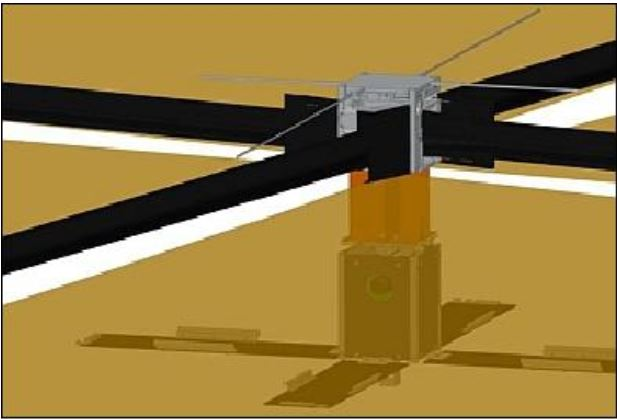
\includegraphics[width=0.5\textwidth]{images/satellitesail.JPG}\\
  \end{center}
  \caption{Deployable booms attached to the solar sails used in DeOrbitSail from source \cite{ESA}}
  \label{fig:sail}
\end{wrapfigure}

The market for small satellites has been growing due to their fast development times, relative low cost of development, compatibility to launch with multiple launchers and the capability to deploy in multiple constellations. However the ever increasing mission requirements often are in contradiction to the mass and volume constraints which are subject to the satellite. Many systems such as solar panels, telescopes, solar sails etc. are in need of reliable deployment of structural booms and arrays for power generation, communications and scientific systems and deployable structures are a solution to that problem. Deployable structures like the one shown in figure \ref{fig:a12} can change their shape and size from a compact configuration to a large, open configuration. 
\begin{wrapfigure}{l}{0.45\textwidth}
  \begin{center}
    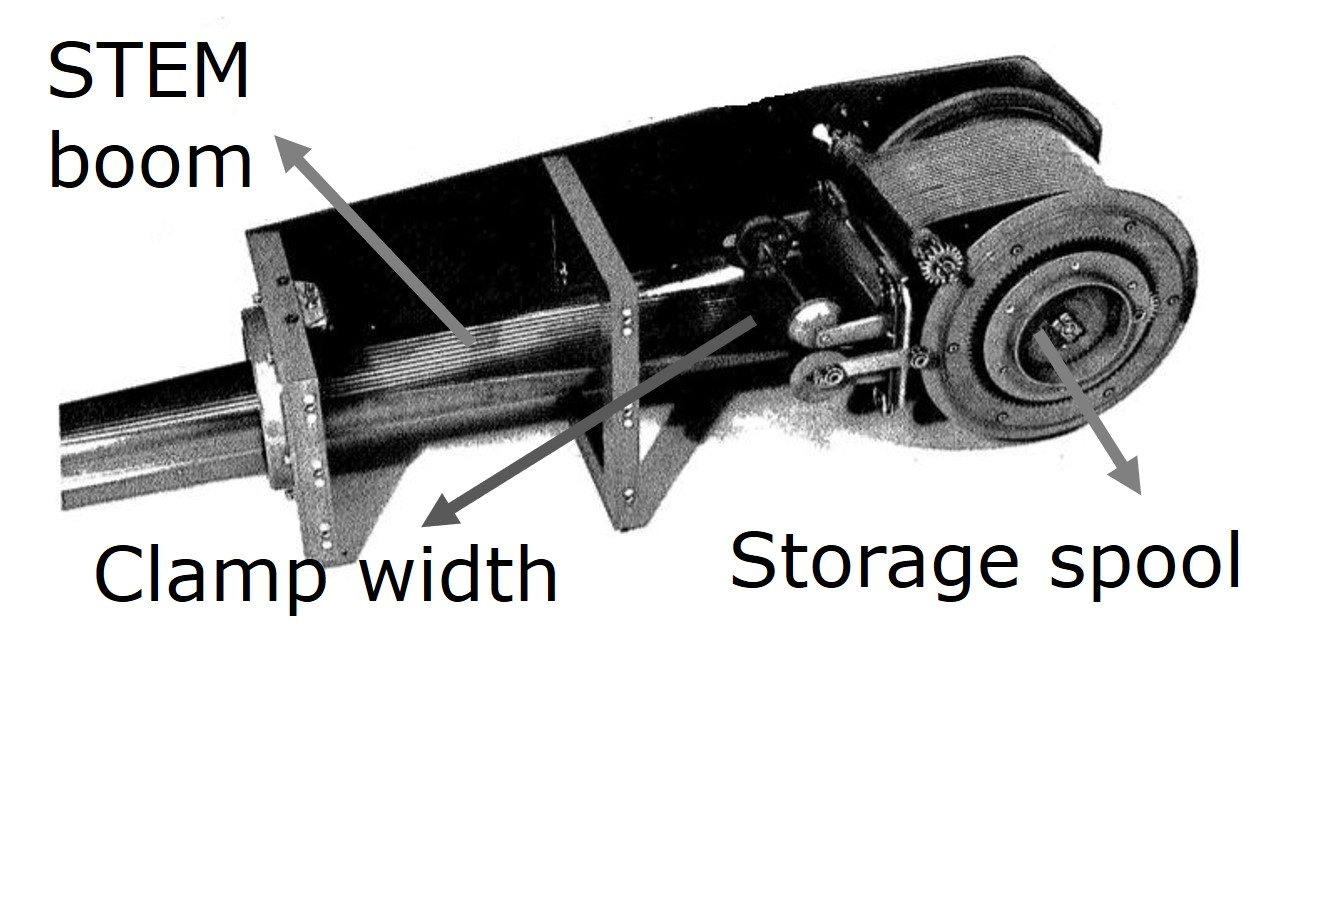
\includegraphics[width=0.45\textwidth]{images/deployerboom.jpg}
  \end{center}
  \caption{A-12 deployer for STEM boom used in apollo missions \cite{NASA}}
  \label{fig:a12}
\end{wrapfigure}
Using the example of the DeOrbit sail satellite developed by the European Space Agency (ESA) \cite{ESA}, deployable booms support a sail in the deorbiting phase of the mission. In the de-orbit stage, compressive loading would be applied to the tip of the boom by the sail due to force of the atmosphere on the sail. However, this can lead to buckling of the boom after surpassing its limit, in which case the sail would fail. Thus, accurate estimates of this limit is vital for the technology to be used. This can be achieved using finite element analysis (FEA) in which the conditions found in space can be replicated. To ensure accurate modelling of the problem in FEA, the boundary conditions of the boom at the root should be modelled accurately. The booms are attached to a satellite deployer shown in figure \ref{fig:a12} using screws spaced apart which ensure that the boom can roll up on the spool. This ensures the deployment of the boom in an aligned and controlled manner. However, in FEA simulations across literature, predominantly an encastered root condition has been applied at the root which can lead to differences in the properties of the boom, since in the actual application the boom would likely be flattened at the end to an extent as can be seen clearly in figure \ref{fig:a12}. 

Thus the aim of this project is to compare the effects on the bending stiffness and the maximum reaction moment of a boom with varying widths of the attachment screws. This is implemented using an analytical model developed and analysed in ABAQUS FEA software \cite{ABAQUS}.     

The literature review in section \ref{sec:litreview} gives an overview of deployable structures, computational models and tape spring behaviour. The methodology in section \ref{sec:method} describes the development of the FEA model of the boom. Results and discussions in section \ref{sec:results} analyses the plots of the lateral displacement, reaction moment, bending stiffness and ploy length. Finally the conclusion in section \ref{sec:conclusion} outlines the future work possibilities of the project. 

\newpage
    \section{Literature review}
\label{sec:litreview}
The following literature review gives an overview of existing deployable booms developed, computer simulations used to model these booms and an explanation of moment rotation curves. 
\subsection{Examples of deployable structures}
% trac boom 
%STEM
\begin{wrapfigure}{l}{0.5\textwidth}
  \begin{center}
     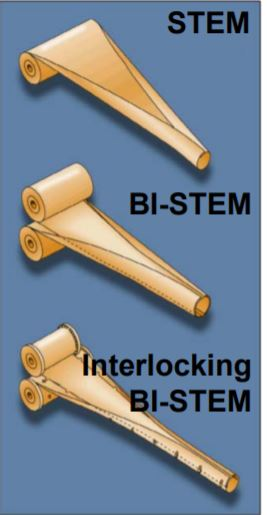
\includegraphics[width=0.3\textwidth]{images/stemderivatives.JPG}
  \end{center}
  \caption{STEM boom and its derivatives image obtained from source \cite{NorthropGrumman}}
  \label{fig:boom}
\end{wrapfigure}
The first type of deployable structure used in space was the Astro Aerospace Storable Extendible Tubular Member (STEM) \cite{NorthropGrumman}. Flown since the 1960's it has proven flight heritage which includes applications on the Voyager spacecraft and the Apollo missions to the moon \cite{NorthropGrumman}. The STEM is a boom with a curved cross section shown in figure \ref{fig:boom}. It rolls up flat on a drum returns to its circular shape after deployment\cite{NorthropGrumman}. The stowed STEM fits into a small space and can be used to deploy/retract other structures like Antennas, Telescopes, Solar array support structure etc. The STEM booms have a simple mechanism and is lightweight. However it has low torsional stiffness and has the tendency to buckle under compression. 
%BI-STEM
A derivative was created to make the booms torsionally stiffer called the BI-STEM booms also shown in figure \ref{fig:boom}. This design includes the use of two STEM booms, one over the other. Because of a closed circular section this type has a higher torsional stiffness which makes it less susceptible to buckling under compression. Further when the STEM booms are being deployed they cause dynamic instabilities in the spacecraft. A BI-STEM boom solves this problem as the two boom motors effectively counter torque each other to provide dynamic damping\cite{Thomson2018}. However this design needs a bigger volume to stow. The loading capability and buckling resistance is limited by the packaging restrictions of these type of booms. Novel methods such as in-orbit bonding of BI-STEM booms are proposed by Schmidt et. al.\cite{Tilo}. 
%CTM
The Collapsible tube mast (CTM) boom \cite{dlr} consists of two laminated sheets which are bonded at the edges to form a tubular shape as shown in figure \ref{fig:ctm}. In the deployment phase the boom is flattened and coiled up on a central hub for storage. During the deployment phase, once the booms are uncoiled they reach their full stiffness by enlarging to its original circular shape. The cross sectional shape gives the boom additional bending stiffness which overcomes the shortcoming of the open cross section of the STEM booms \cite{Fernandez2017}. Thus for the same deployed diameter, the CTM boom has half the packaged height as the STEM and requires less strain to flatten \cite{Murphey2011}. However due to prolonged stowage, significant cross section flattening was observed \cite{Fernandez2017} which reduced the load bearing capacity by 50\%. 
\par
%tapespring
More recently, developed for the deployable mechanisms of satellite de-orbiter, CopperBeryllium (CuBe) tape springs offer an alternate solution \cite{Fernandez2013}, which look like STEM booms shown in figure \ref{fig:boom}. Two CuBe springs face each other to form a lenticular cross-section. The two tape springs are then encased by a Kapton sheath to form a closed cross-section with an improved torsional stiffness and buckling load. As the booms are coiled for storage, the two tape springs will slide with respect to each other inside the Kapton sheath, thereby reducing the amount of shear stress and strain energy stored in the stowed configuration. \cite{Fernandez2013}
%BRC
The Rolatube used in Inflatsail satellite in 2017\cite{Rolatube} in an example of bistable reeled composites which are stable in both deployable and stowed configuration due to their composite laminate design. Due to this property, these type of booms dont require a restraining device, however it is often in practice that satellites carry a motor to deploy these booms in order to control the deployment of the booms. 
%multiangle braids
Carbon fibre booms in a coiled state experience high strains which can cause delamination and creep effects on the material \cite{Fernandez2013}. The Open section CFRP booms utilise an interesting innovation to reduce the high strain during the stowed configuration. By varying the braid angle quasi-linearly from root to tip (respectively 50\degree and 35\degree), the natural coiling radius will vary linearly along the boom length, and the boom will thus coil into an Archimedean spiral \cite{Fernandez2013}. This ensures that the four co-coiled booms will be in their lowest energy state possible and in a stable configuration, and no edge buckling will take place. Creep effects during long term storage are also reduced with this approach. 
%shearless
\par
\begin{wrapfigure}{r}{0.5\textwidth}
  \begin{center}
     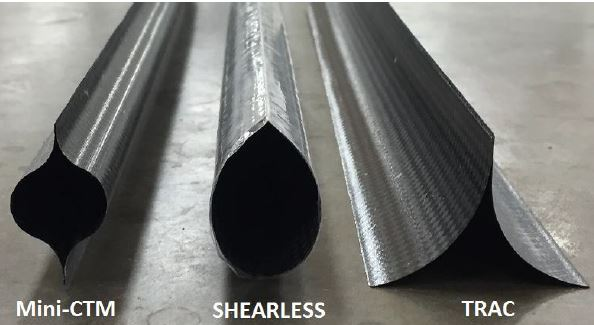
\includegraphics[width=0.48\textwidth]{images/ctmshearless.JPG}
  \end{center}
  \caption{CTM, SHEARLess and TRAC booms \cite{Fernandez2017}}
  \label{fig:ctm}
\end{wrapfigure}
SHEAth-based Rollable LEnticular-Shaped and low-Stiction (SHEARLESS) boom \cite{shear} is fabricated from joining two independent tape-springs front-to-front with the use of a durable seamless polymer sleeve. This sleeve allows the two parts to slide past each other during the coiling/deployment process so as to minimize shear and its derived problems. And during storing of the boom, it first flattens and then the two tape springs axially slide against the polymer. Thus the shear stresses are endured by the flexible sheath rather than the bond line. The main advantage of this design is that it reduces tendency of the inner shell undergoing compression to buckle locally giving an improvement over the TRAC and CTM booms with little increase in mass or complexity \cite{Fernandez2017}. The sheath encloses and couples the two inner shells so there are no problematic adhesive bonds in the design and long term stowage creep effects are thus reduced. As in CTM designs, the doubly-symmetrical cross-section of the SHEARLESS boom makes the centroid (neutral axis) and the shear center coincident. This eliminates undesired flexural-torsional coupling that can often cause buckling and collapse in torsionally weak slender booms like these.\cite{Fernandez2017} However the current challenge is computational modelling of the SHEARLESS booms as they give largely non linear responses.\cite{Fernandez2017}
%TRAC 
\par
The US Air Force Research Laboratory developed the Triangular Rollable and Collapsible (TRAC)  boom shown in figure \ref{fig:boom}. This boom is made of two curved C-shaped sections joined along one edge \cite{Murphey2011}. This results in a large cross-section inertia to packaged height ratio compared to STEM and CTM architectures \cite{Murphey2011}. Even though this design reduces the torsional stiffness of the boom, bending stiffness is the limiting measure of performance for most applications\cite{Murphey2011}. In addition, the strain required to flatten the flanges of a TRAC boom are smaller than the STEM or the CTM booms allowing for thicker flange materials to be used \cite{Murphey2011}. This results in greater bending stiffness as compared to the aforementioned boom types. Predicted performance of the TRAC boom indicate 10 times greater bending stiffness than a CTM boom with the same packaged height and material and 34 times greater bending stiffness than a STEM boom \cite{Murphey2011}.
%Bi-TRAC
\par
TRAC booms which are bi-stable in both deployed and stowed configurations are called Bi-TRAC booms. The inner shell of the beam is made with a Bi-stable laminate and the outer shell is made with a less stiff laminate with a larger strain to failure capacity. The main advantage of the bi-TRAC boom is its more predictable and controlled deployment dynamics from coiled to deployed state. For example, a 0.3m Bi-TRAC boom can take 6-8s to self deploy compared to tenths of seconds a TRAC boom would take. Thus it would be a lighter and less complex mechanism.

In summary the following deployable booms have been discussed as given in the table below.  
\begin{table}[!hbt]
\centering
\begin{tabular}{|l|l|}
\hline
\textbf{\begin{tabular}[c]{@{}l@{}}Deployable boom type\end{tabular}} & \textbf{Key features} \\ \hline
STEM & \begin{tabular}[c]{@{}l@{}}Deployable, lightweight, small\\ Low torsional stiffness \\ Low buckling stiffness\end{tabular} \\ \hline
Bi-STEM & \begin{tabular}[c]{@{}l@{}}Higher torsional stiffness\\ Counter torque when deployed\\ More volume to stow\\ Non interlocked tapes\end{tabular} \\ \hline
CTM & \begin{tabular}[c]{@{}l@{}}Half the packaged height\\ Requires less strain to fold\\ Flattening of boom causes less load bearing capacity\end{tabular} \\ \hline
TRAC & \begin{tabular}[c]{@{}l@{}}Higher bending stiffness \\ Strain required is lesser\end{tabular} \\ \hline
Bi-TRAC & More stable when self deploying \\ \hline
SHEARLess & \begin{tabular}[c]{@{}l@{}}Higher buckling resistance\\ 2 tape booms are enclosed by a sheath\end{tabular} \\ \hline
\end{tabular}
\caption{Summary of deployable structures}
\end{table}
\begin{comment}
Oxford space systems have developed ASTROTUBE\texttrademark \hspace{0.1 cm} BOOM which supports a wide range of Microsat and cubesat application \cite{Oxfordspacesystems}.They have also been flight proven on the AlSat-Nano3U cubesat \cite{Oxfordspacesystems}. The boom element can be fully or partially deployed which is a result of a greater control of the deployment sequence as compared to the rollable booms. \cite{EoPortal}.
\end{comment}
\subsection{Computational modelling}
A computational modelling approach is selected in this report in order to study the effects of boundary conditions to better model conditions found in space, where the booms are meant to operate in. An overview of the computational models of STEM booms are given. These techniques are later used in the model developed for this paper. 
%boundary conditions etc. 
%BRC
Dynamic analysis of a cantilevered boom BRC attached to solar sails was conducted in FE package ABAQUS by Wu et. al \cite{Wu2018}. The Budiansky Hutchinson criteria\cite{Budiansky} was used to find the instability criteria based on changes in cross section. It was found that the buckling occurs at different accelerations for same sense bending and opposite sense bending, with the same sense bending occurring faster. The spacecraft was assumed to be a rigid square plate to which an extended Bistable reeled composite (BRC) is attached. 
One end of the BRC boom is tied rigidly to the square plate using a 'Master Slave' algorithm in ABAQUS. For the loads modelling an angular acceleration is used. S4R shell elements with reduced integration to model the composite booms as they are robust and have a lower computational cost. 
The Budiansky-Hutchinson criterion \cite{Budiansky} for shell structures which states that dynamic stability loss occurs when the maximum deflection grows rapidly with the small variation of the load amplitude is used to estimate the critical angular acceleration that booms can sustain before becoming unstable during a spacecraft's rotational manoeuvre. 
The cross-section deformation in the transverse direction, $\xi$ is used as the key parameter to estimate the maximum angular acceleration. To validate the experiment, the behaviour of a boom in microgravity is extremely difficult however it is possible to simulate the g value in linear acceleration.
A laser distance gauge was used to measure the end displacement of the boom. A correlation with an approx 5.9\% difference was found between the experimental and simulated tip displacement. 
This result was used to verify the bending reliability of the FE simulation. Using the Budiansky-Hutchinson criterion the critical rotational acceleration can be found for the single boom and validated against the FE results. However in this paper it is assumed that the base of the boom connected to the satellite would have all 6 degrees of freedom constrained with no change in geometry \cite{Wu2016}. This end condition is not representative of the satellite deployer attachment and can give inaccurate results.
\subsection{Moment rotation curve}
\begin{figure}[!hbt]
    \centering
     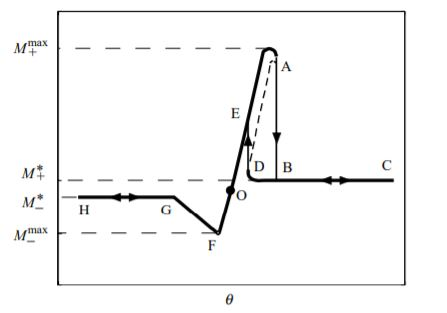
\includegraphics[width=10cm]{images/tapespring.JPG}
     \caption{Tape spring reaction moment vs rotation curve \cite{Seffen1999}}
  \label{fig:tapetheory}
\end{figure}
Tape springs have the same moment vs rotation curve as that of the STEM booms. The non-linear behaviour exhibited by them are studied in this overview which are used to explain the results obtained in section \ref{sec:results}. 
The figure \ref{fig:tapetheory} shows the relationship between the reaction moment and the rotational moment of a tape spring where point O is the neutral point where no displacement is applied. A positive moment in this case is referring to opposite sense bending and a negative moment is referring to same sense bending shown in figures \ref{fig:same} and \ref{fig:opp}. 
As the same sense bending moment is applied to the tape spring, the curve linearly progresses to the point F after which it snaps and the propogating moment stays constant for increase in $\theta$. If a negative moment is applied, the linear behaviour ends much sooner. At point F there is a sudden snap that results in a flexural-torsional deformation mode with a formation of a fold \cite{Seffen1999}.
From this point onwards M remains constant as $\theta$ is further increased (points G to H) \cite{Seffen1999}. When $\theta$ is decreased, the unloading path practically coincides with the loading path \cite{Seffen1999}. It can be seen that the peak moment for same sense bending is lesser than the peak bending moment of the opposite sense bending because the flexural-torsional mode of failure in the same sense bending occurs sooner than the buckling mode of failure in the opposite sense bending \cite{Seffen1999}. 
In reference \cite{Seffen1999}, it is mentioned that an elastic fold developed that is sufficiently far away from the ends of a tape spring consists of two symmetric transition regions on either side of a cylindrical region with uniform curvature \cite{Seffen1999}. The angle subtended by this cylindrical region is approximately equal to the relative rotation $\theta$ between the ends of the tape spring, as both the transition regions and the remaining parts of the tape spring have negligibly small longitudinal curvature \cite{Seffen1999}.
It has been shown that in the absence of end effects the bending moment at the fold remains approximately constant as $\theta$ varies \cite{Seffen1999}. 
This behaviour changes when the fold reaches near the built-in end, where the cross-sectional shape is held rigidly fixed. Here the fold stops moving but only $\theta$ can change. 

    \section{Methodology: Finite element analysis}
\label{sec:method}
A FEA model was created in ABAQUS. The geometry is based on dimensions obtained from reference \cite{Wu2018}, with a length of 500mm and a subtended angle of 90\degree. The shell element was extruded with a thickness of 0.1mm. Copper Berrilium was chosen as the material with youngs modululus (E) of 156 GPa \cite{Azomaterials} and a poisson' ratio ($\nu$) of 0.35 \cite{Azomaterials}. A mesh refinement study was conducted, after which the 0.0001m mesh size was chosen using the cantilever displacement as a test against the analytically derived result. The mesh elements were formed using S4R elements. To flatten the boom at the root, the equation \ref{eq:disp} was used to find the displacement needed at every node have a flat row of nodes.
\begin{equation}
  y=R-R\times cos(\theta)  
  \label{eq:disp}
\end{equation}
Where $\theta=\frac{Width}{Radius}$. 
Figure \ref{fig:rootdisp} shows the image of the displacement conditions at the tip. Displacement conditions applied resulting in fully flat section as shown in \ref{fig:case24}. The different widths of the booms are modelled by suppressing the nodes from the outer width. Since there were 48 nodes in the root section, the mesh size across the root was calculated by dividing from the circumference of the root end of the boom. 
%table for summary of properties 
These displacements are further given in appendix. In order to find the effects on the boom for the displacement used, the rotational displacement against the moment observed were used to depict on a graph. This was found by constraining the tip nodes using a single control point via a Multi Point Constraint (MPC) and a beam constraint was used in order to equally apply displacements on the tip. The reference point for the node was set at the centre of the semi circle which was used to apply the rotational condition.  

\begin{table}[!hbt]
    \centering
    \begin{tabular}{|c|c|c|c|c|c|}
    \hline
    \textbf{Length} & \textbf{Thickness} & \textbf{Radius} & \textbf{Meshsize} & \textbf{\begin{tabular}[c]{@{}l@{}}Young's\\ Modulus\end{tabular}} & \textbf{\begin{tabular}[c]{@{}l@{}}Poisson's\\ Ratio\end{tabular}} \\ \hline
    500mm & 0.1mm & 15mm & 0.1mm & 158GPa & 0.35 \\  \hline
    \end{tabular}
    \caption{Summary of FEA model}
    \label{tab:fea}
\end{table}
\begin{figure}[!hbt]
\begin{subfigure}{.5\linewidth}
\centering
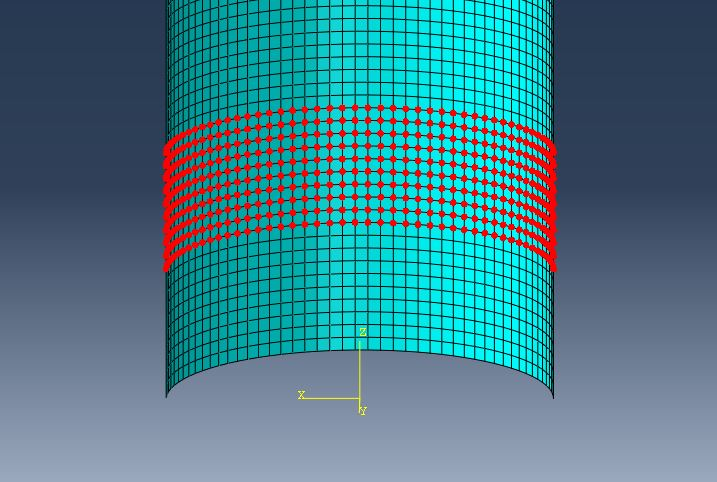
\includegraphics[height=5cm]{images/RootDisp.JPG}
\caption{Displacement conditions required to make the end flat}
\label{fig:rootdisp}
\end{subfigure}%
\begin{subfigure}{.5\linewidth}
\centering
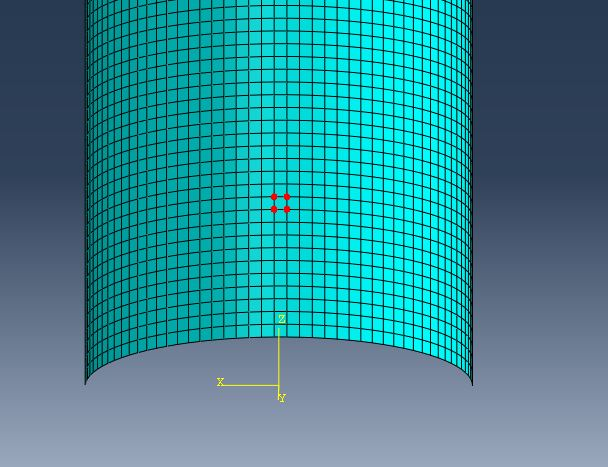
\includegraphics[height=5cm]{images/encastre.JPG}
\caption{Fixed nodes at the root}
\label{fig:sub2}
\end{subfigure}\\[1ex] 
\caption{Displacement conditions applied at the root}
\end{figure}

\begin{figure}
\begin{subfigure}{0.5\linewidth}
\centering
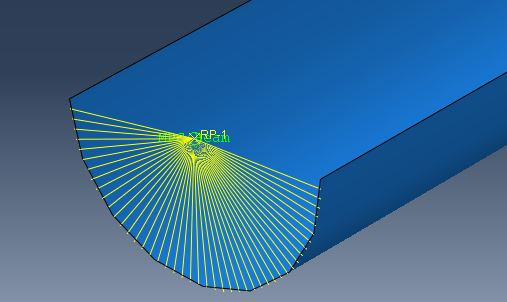
\includegraphics[width=7cm]{images/connectorMPCbeam.JPG}
\caption{MPC connector beam tie linking the nodes in the arc to the reference point using a `Master-Slave' algorithm}
\label{fig:sub3}
\end{subfigure}
\label{fig:test}
\begin{subfigure}{0.5\linewidth}
\centering
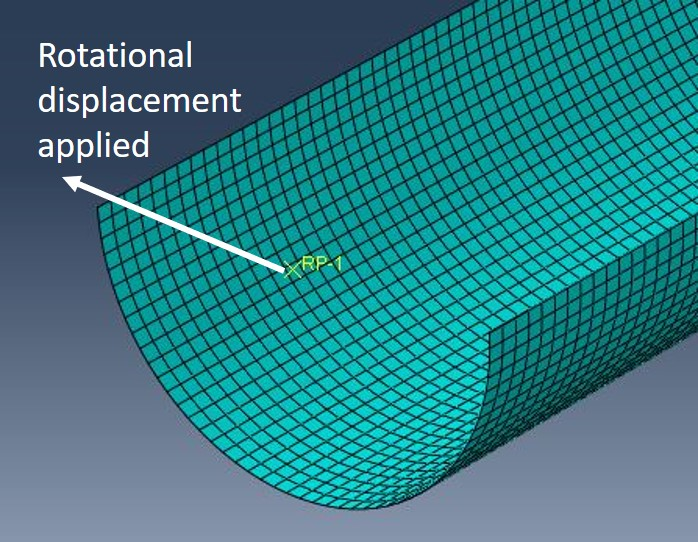
\includegraphics[width=6cm]{images/RP12.jpg}
\caption{Rotational displacement applied to the reference point at the centre of the semi circular arc}
\label{fig:sub3}
\end{subfigure}\\[1ex]
\caption{ABAQUS model tip properties}
\label{fig:test}
\end{figure}

    \newpage
    \section{Results and Discussions}
\label{sec:results}
The following section presents and discusses the results for this project namely the ploy length parameter and  bending stiffness of the boom derived with respect to change in the clamp width. These results would be used to explain the results obtained in the bending and flattening cycles of the booms with different clamp widths, one example of which is shown in figure \ref{fig:sequence}. 
%seq for deformation. 
\begin{figure}[!hbt]
\begin{subfigure}{.5\linewidth}
\centering
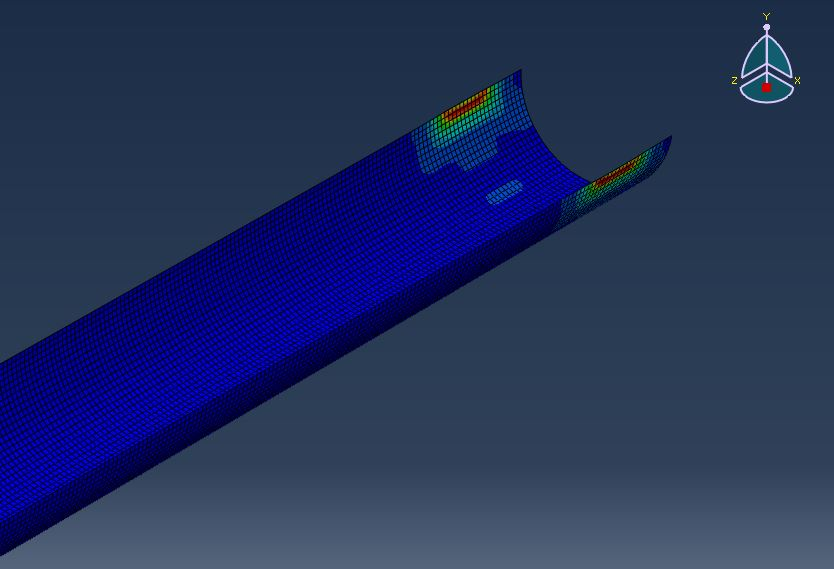
\includegraphics[height=4.5cm]{images/1.JPG}
\caption{}
\label{fig:sub1}
\end{subfigure}%
\begin{subfigure}{.5\linewidth}
\centering
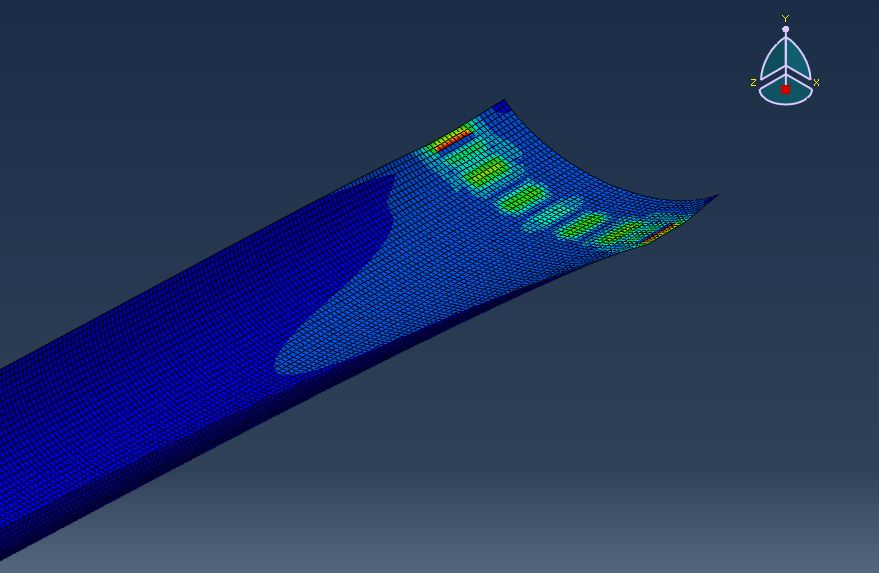
\includegraphics[height=4.5cm]{images/3.JPG}
\caption{}
\label{fig:sub2}
\end{subfigure}
\begin{subfigure}{.5\linewidth}
\centering
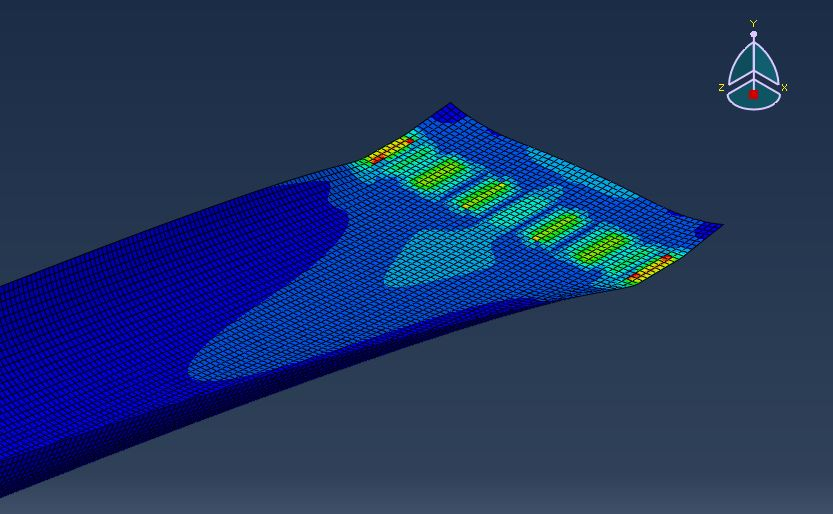
\includegraphics[height=4.5cm]{images/4.JPG}
\caption{}
\label{fig:sub3}
\end{subfigure}
\label{fig:test}
\begin{subfigure}{.5\linewidth}
\centering
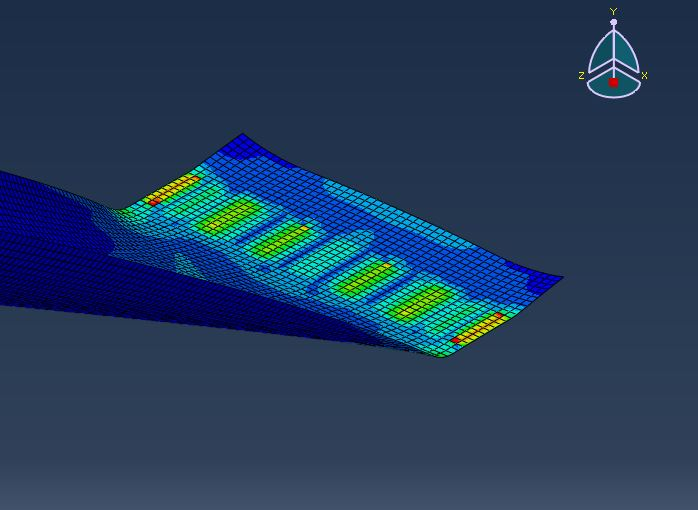
\includegraphics[height=4.5cm]{images/6.JPG}
\caption{}
\label{fig:case24}
\end{subfigure}
\caption{Sequence of flattening of the root and bending of a fully clamped boom in ABAQUS in order (a) to (d)}
\label{fig:sequence}
\end{figure}

\subsection{Lateral displacement}

% need fig 1 before text? or some intro at least? 
Figure \ref{fig:ploy1} shows a plot showing the deformed width of the boom along the length with different clamp widths at the root of the boom. It is observed that the maximum lateral width of the boom increases with an increase in width of the root clamp, which can also be observed in figure \ref{fig:ploydefine}. 

\begin{figure}[!hbt]
    \centering
    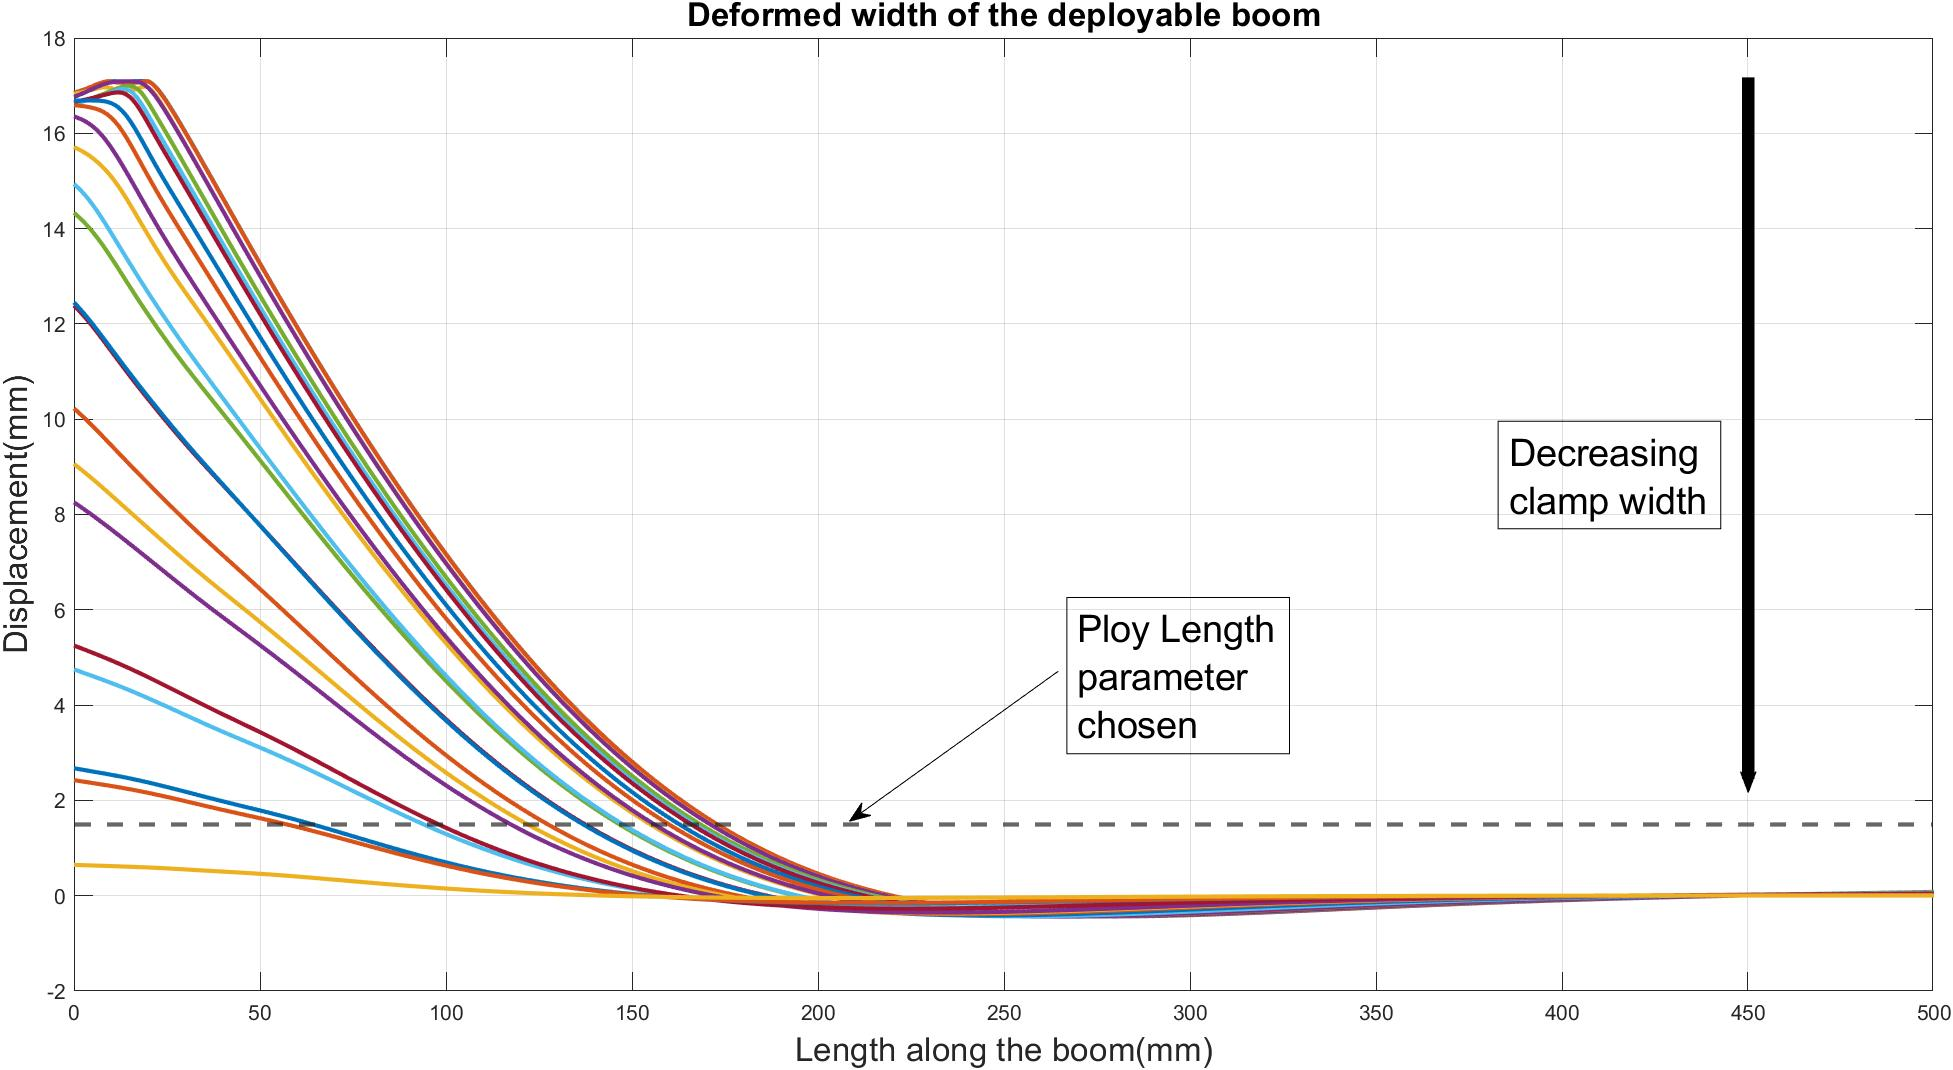
\includegraphics[width=15cm]{images/maxwidth.jpg}
    \caption{Deformed width of boom compared to the length of the boom}
    \label{fig:ploy1}
\end{figure}

Interestingly, it is also observed that the tape bends slightly inwards around the middle of the boom thus giving a negative displacement. However the maximum limit of this negative displacement is nearly constant at -0.44mm. Further, the different cases return to null displacement at nearly the same length. This is shown more clearly in the figure \ref{fig:negdisp}.   

\begin{figure}[!hbt]
    \centering
    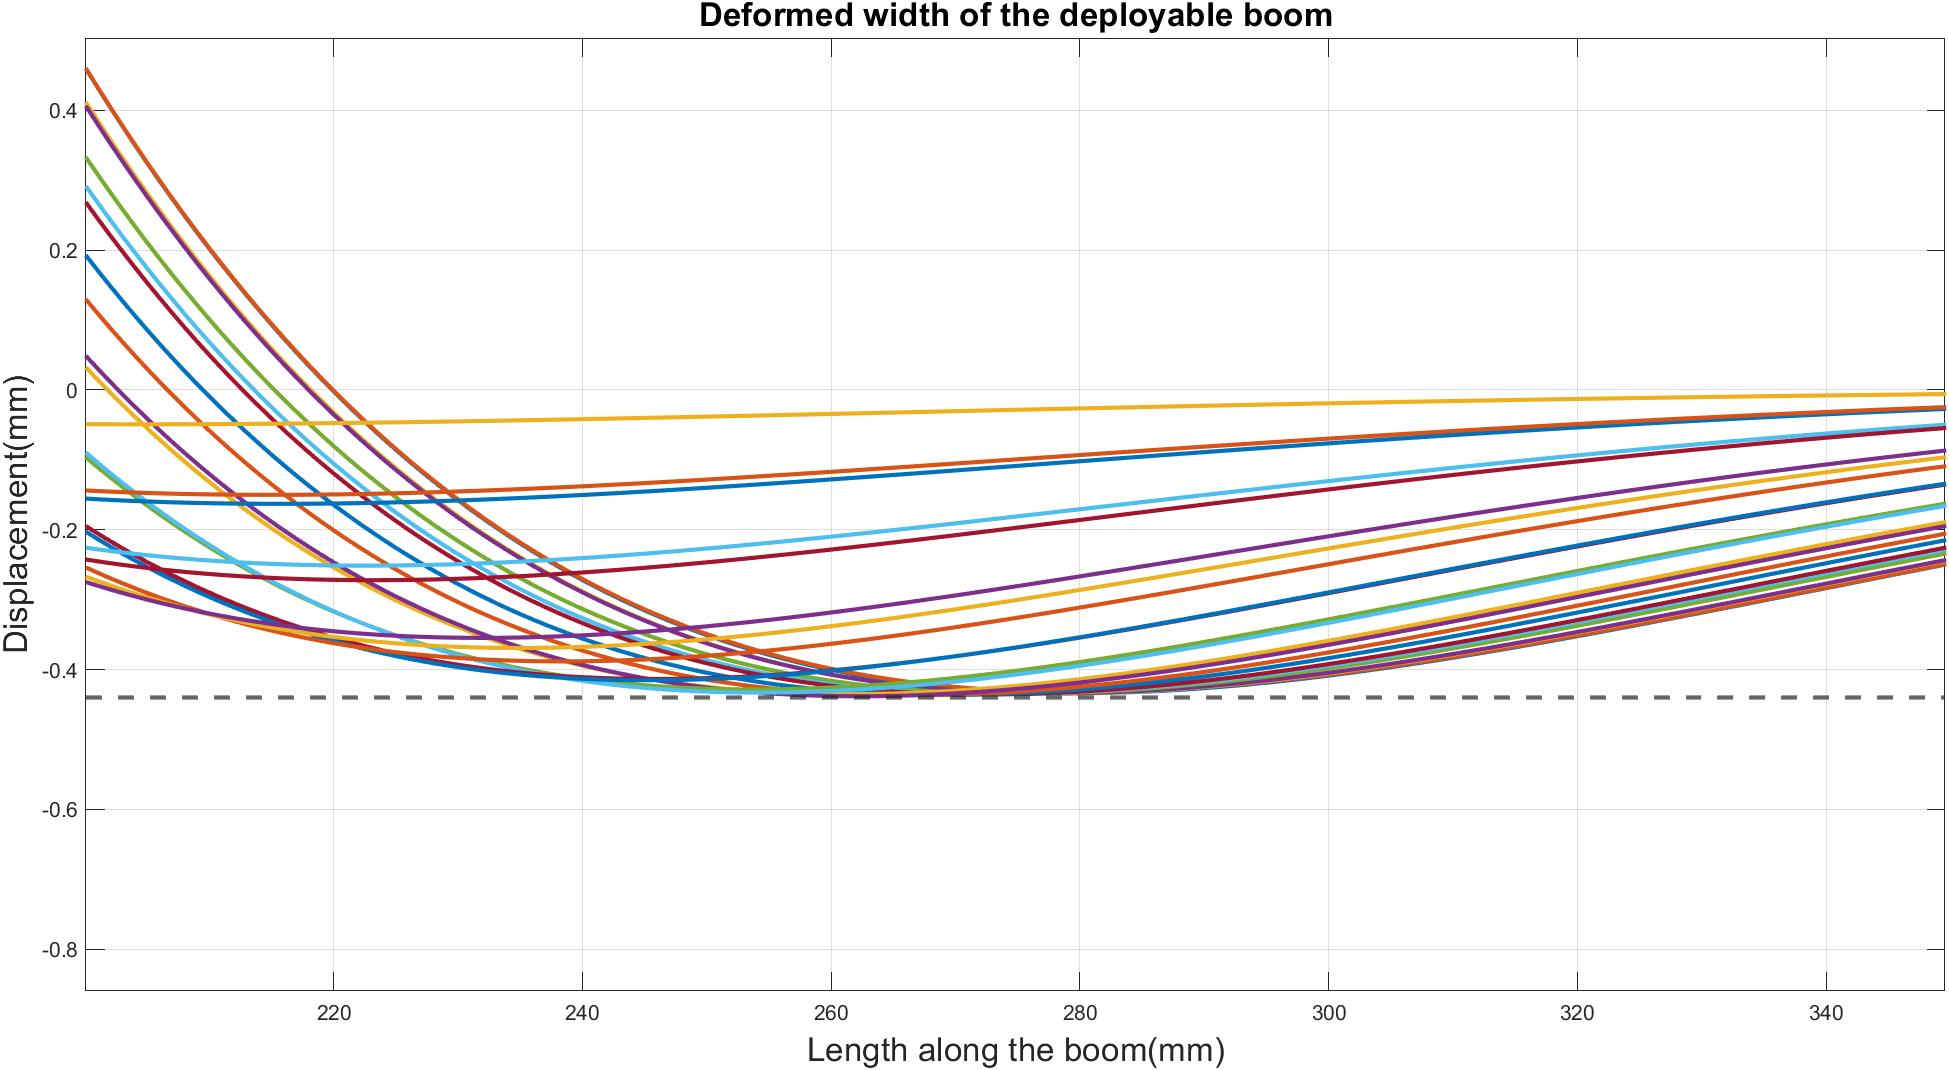
\includegraphics[width=15cm]{images/zoomin.jpg}
    \caption{Negative displacement}
    \label{fig:negdisp}
\end{figure}
\subsection{Ploy length parameter}
Figure \ref{fig:ploydefine} shows the deformed boom once the boundary conditions were applied in FE software ABAQUS. After flattening of the boom, the boom returns to its original curvature further along the distance. The ploy legnth parameter is the distance along the boom from the clamp where it is flattened to where the lateral width of the deformed boom is nearly equal to the lateral width before the deformation. In this paper, it is selected to be 5\% deviation of the undeformed width of the boom. The ploy length is an important result as this later helps in the design of a STEM boom deployer, by allowing for the positioning of guide rollers to ensure smooth deployment of the boom and keeping its alignment shown in figure \ref{fig:guiderollers}. 
\begin{figure}[!hbt]
    \centering
    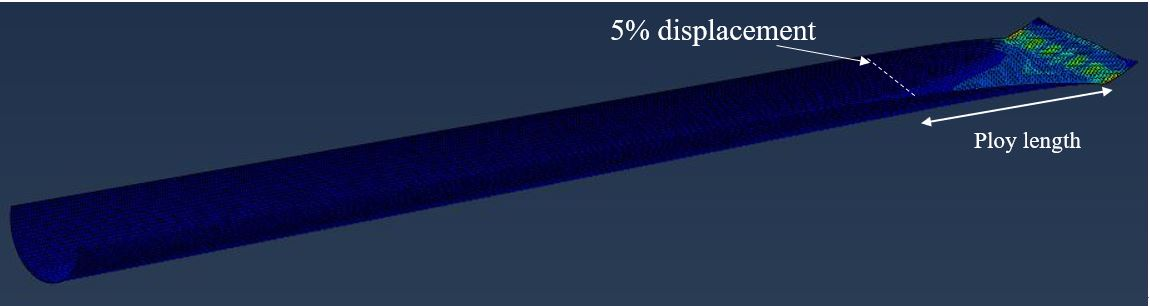
\includegraphics[width=15cm]{images/pic1.JPG}
    \caption{Ploy length}
    \label{fig:ploydefine}
\end{figure}

\begin{figure}[!hbt]
    \centering
    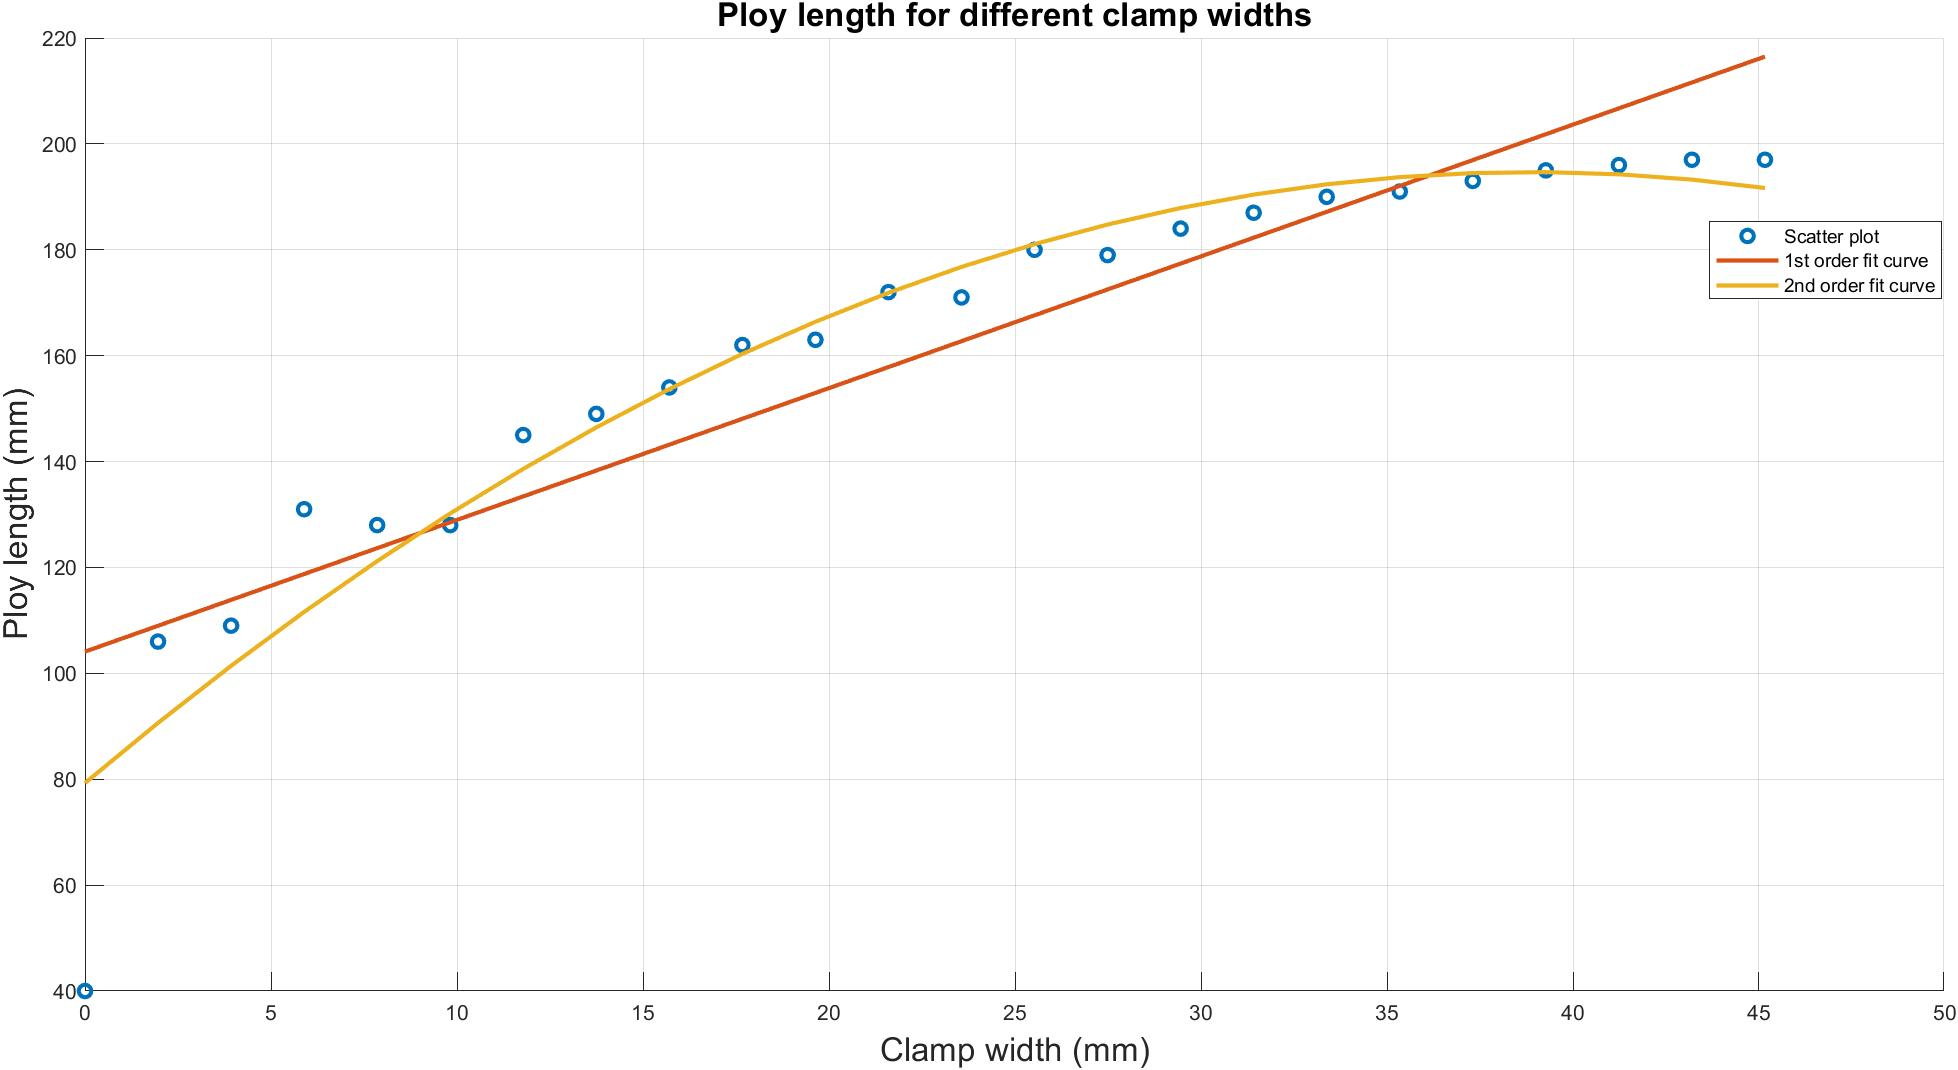
\includegraphics[width=15cm]{images/fitcurve.jpg}
    \caption{Ploy length second order fitted curve}
    \label{fig:fitcurve}
\end{figure}
In figure \ref{fig:fitcurve}, the scatter points are the ploy lengths of the different cases obtained by using the above mentioned ploy length parameter. Figure \ref{fig:fitcurve} shows the fitting of polynomial curves to the data obtained. In the plot a first order and second order equations are compared with regards to their fit with the data, and it is observed that the second order curve is better suited as a relation curve between the width of the clamp and the ploy length. The equations were obtained using MATLAB's polyfit function. The second order fit for the ploy length $L_{\mathrm{ploy}}$ is given by equation \ref{eq:ployfit}
\begin{equation}
    L_{\mathrm{ploy}}=-0.08 \times W^2+5.93 \times W+79.28
    \label{eq:ployfit}
\end{equation}
where $W$ is the width of the clamp area. 
%definition of ploy length 
The definition of this ploy length was chosen to be 5\% deviation of undeformed lateral width of the boom. Reference \cite{Yang2018} fixes the definition for the ploy length to be 5\% deviation in the curvature of the boom, however for the purposes of the report the length parameter is chosen. In this case, a 5\% deviation of the diameter of 30mm is 1.5mm.  A plot comparing different definitions is given in figure \ref{fig:ploydef}, which shows that the different even if a parameter for 10\% or 15\%  was taken, the shape of the plot does not change, validating this paper's parameter selection.  
\begin{figure}[!hbt]
    \centering
    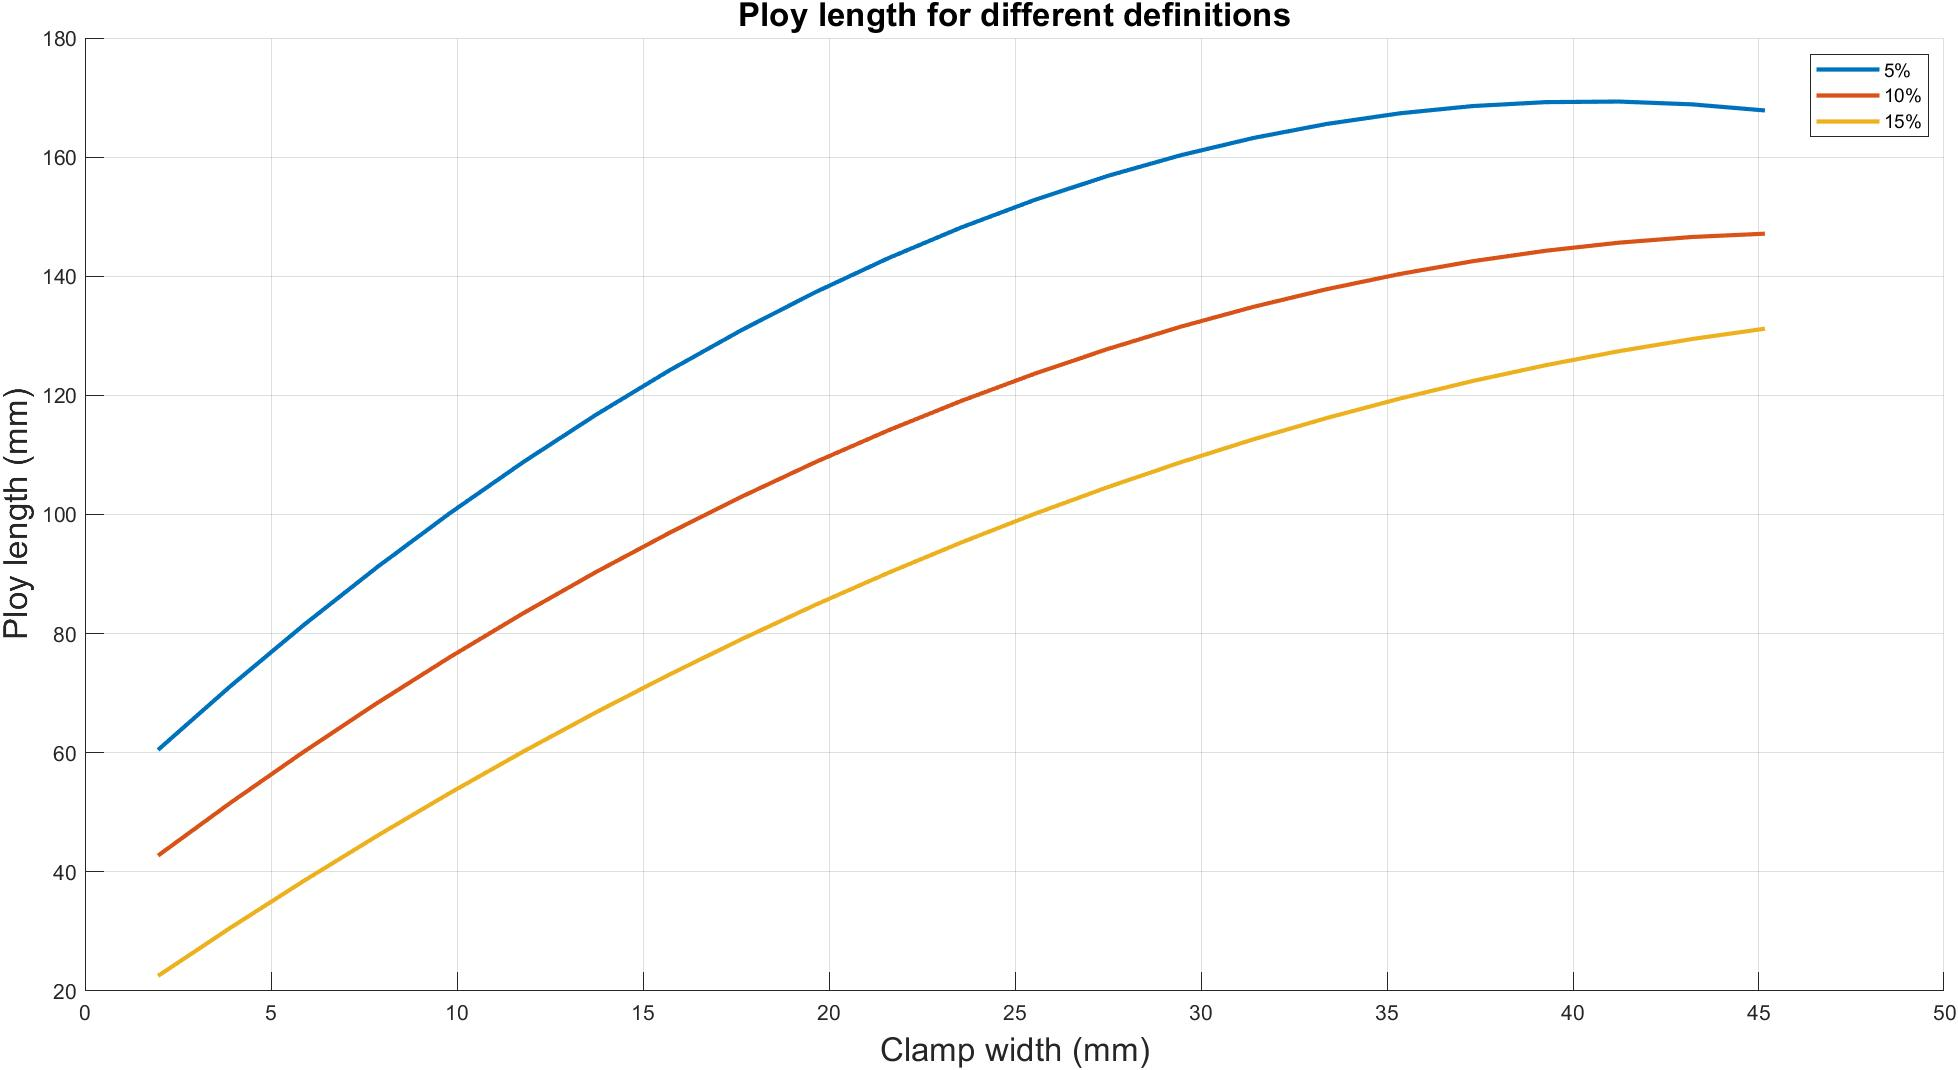
\includegraphics[width=15cm]{images/ploylen_def.jpg}
    \caption{Ploy length plots for different definitions}
    \label{fig:ploydef}
\end{figure}
\subsection{Bending stiffness}
\begin{figure}[!hbt]
    \centering
    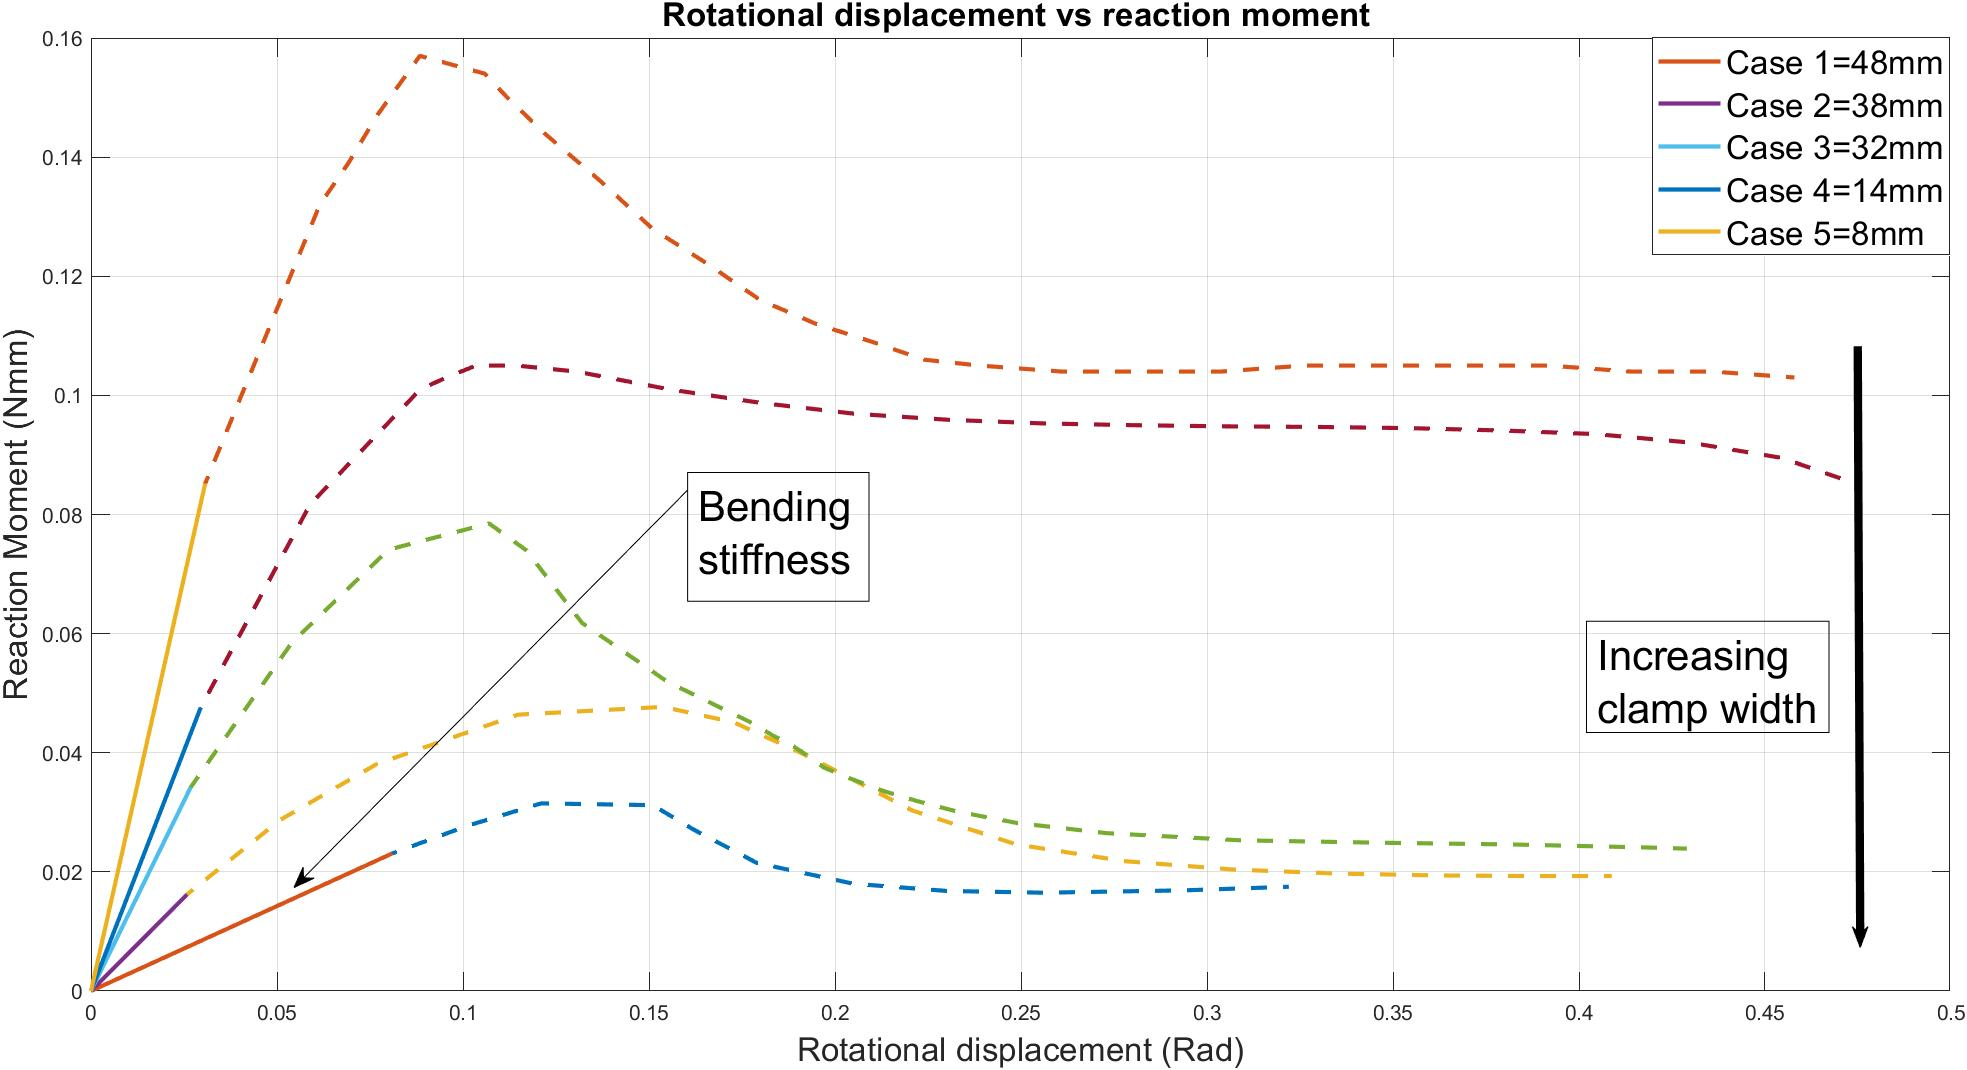
\includegraphics[width=15cm]{images/rotdispupdated.jpg}
    \caption{Rotational displacement plotted against reaction moment for varying clamp widths}
    \label{fig:rotdisp}
\end{figure}
% put a new image without the fitted curve + possibly new data points. 
Figure \ref{fig:rotdisp} shows the relationship between the reaction moment and the rotational displacements for different clamp widths for applied same sense bending. In this plot case 1 is fully encastered whereas case 5 has the least clamp width. The linear slope shown in the plot is used to calculate the bending stiffness of the booms for the different clamp widths in figure \ref{fig:bendstiff}. The curves initially reach a peak maximum reaction moment and thereafter there is a sharp decrease in reaction moment. Once this propagation moment is reached it remains constant for further increase in $\theta$. This is because the boom initially deflects upwards and after reaching the peak moment, it buckles resulting in a sharp decrease in reaction moment \cite{Seffen1999} as can be seen in figure \ref{fig:boom}. This buckling leads to a fold development across the width of the boom as shown in figure \ref{fig:case24} also discussed in the literature review. 
The peak reaction moment and subsequently bending stiffness of the booms increase with a decrease in clamp width. This is because of non-linear fold-support effects on the booms observed in figure \ref{fig:foldint}, which is a plot of peak reaction moments with respect to y/R which is essentially the extent of the fold developed across the boom \cite{Seffen1999}. Comparing figure \ref{fig:case19} which has a clamp width of 38mm and figure \ref{fig:case24} which is fully flat with a clamp width of 48mm, the extent of the fold developed across the boom is different. This is because a narrow clamp has a different transverse curvature to that of the fold. Thus, figure \ref{fig:case19} has a partial fold which results in a higher peak moment for a narrower clamp in figure \ref{fig:rotdisp}. Figure \ref{fig:case24} has a full fold since the boundary condition has the same curvature as that of the fold, and thus its peak moment is lower.
\begin{figure}[!hbt]
     \centering
     \begin{subfigure}[b]{0.4\textwidth}
         \centering
    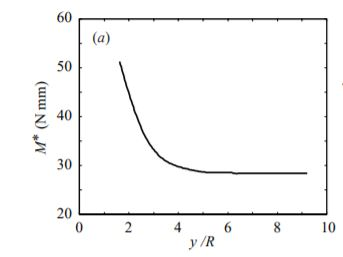
\includegraphics[height=4.5cm]{images/foldinteraction.JPG}
    \caption{Fold interaction with varying y/R from source \cite{Seffen1999}}
    \label{fig:foldint}
     \end{subfigure}
     \hfill
     \begin{subfigure}[b]{0.4\textwidth}
         \centering
    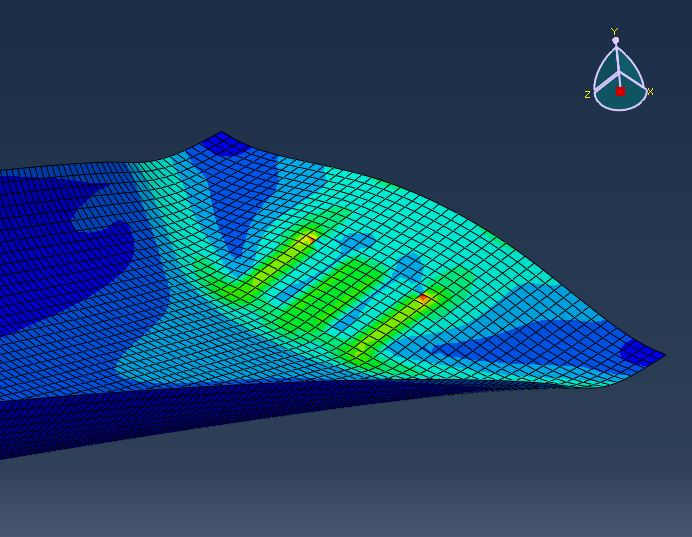
\includegraphics[height=4.5cm]{images/halfwidth.JPG}
     \caption{Fold development in a clamp with narrower width}
  \label{fig:case19}
     \end{subfigure}
     \caption{Fold support interaction}
\end{figure}
%so how does fold influence the bending moment?
A fully developed fold across the boom causes a decrease in energy which results in lowering of the reaction moment and consequently the bending stiffness. Mansfield et. al. have developed a theory for same sense bending based on Calladine's shell theory \cite{calladine_1983} analyzing a strip of constant thickness on a cylinder to be taken as a tape spring. More details are shown in figure \ref{fig:mansfield} in appendix. According to this theory, the equation for longitudinal bending moment, $m_{yz}$ is given by equation \ref{eq:mansfield} from reference \cite{Seffen1999}. 
\begin{equation}
    m_{yz}=D\Bigg[\nu(\dv[2]{u}{z}+\frac{1}{R})+(\frac{1}{r_1})\Bigg]
    \label{eq:mansfield}
\end{equation}
Where, $D=\frac{Et^3}{12(1-\nu^2)}$, $\dv[2]{u}{z}$ is the differential of the height of the tapespring and $\frac{1}{r_1}$ is local curvature at a point. Due to the formation of a flat fold the factor, $\dv[2]{u}{z}=0$ hence there is a significant reduction in bending moment compared to a constrained boom. 
%propogating moment
It is also seen that the propagating moments are different for different clamped widths. It is plausible that due to the above mentioned fold-support interactions the propagating moments increase for a decrease in clamp width. 
\begin{figure}[!hbt]
    \centering
    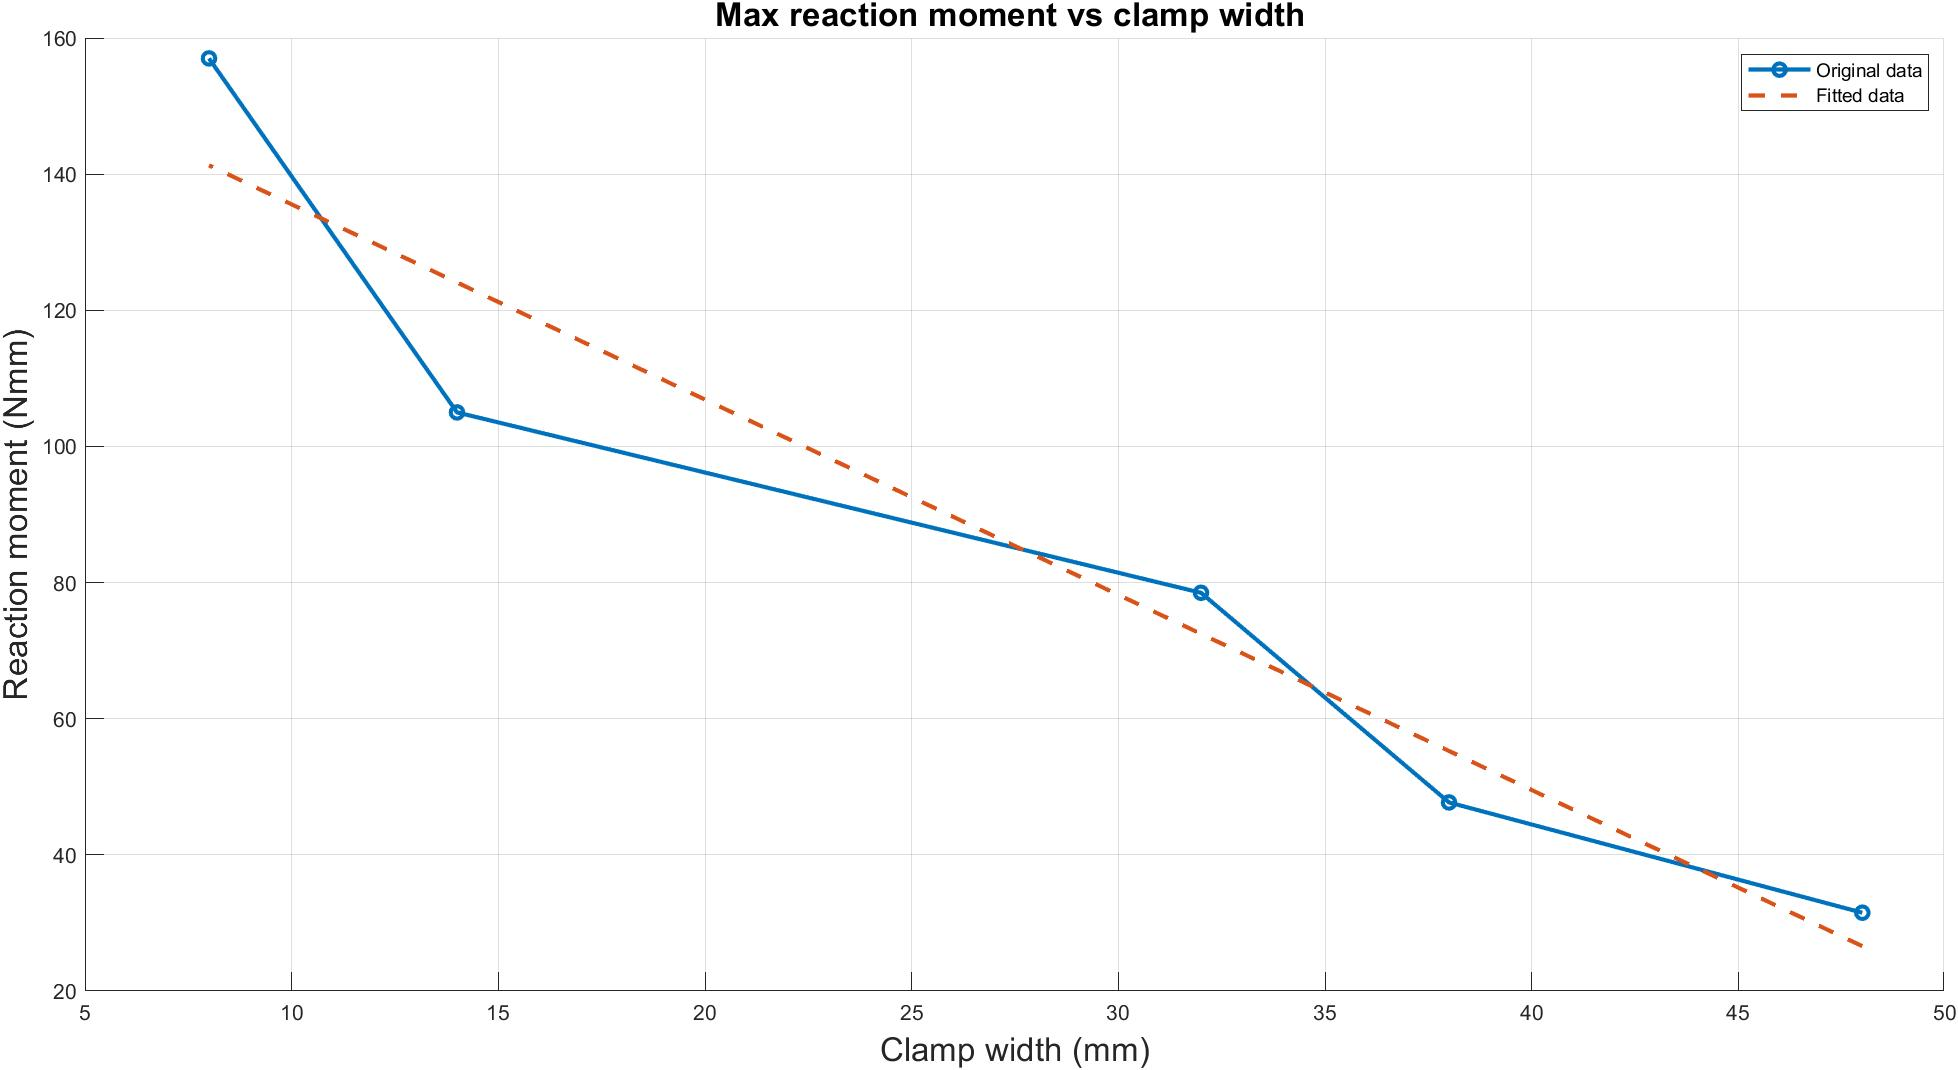
\includegraphics[width=15cm]{images/maxRM.jpg}
    \caption{Fitted curve for the plot between the maximum reaction moment and clamp width}
    \label{fig:maxRM}
\end{figure}
The following plot shows the relationship between maximum reaction moment for differing clamp widths. The correlation factor of the two variables is given by -0.9624 indicating a strong linear negative correlation between the two variables. Thus when the width increases the rotational moment decreases and vice versa. A linear curve is fitted across the data to give the following plot with the following equation, where $R_{\mathrm{max}}$ is the maximum reaction moment and W is the width of the clamp width.   
 \begin{equation}
     R_{\mathrm{max}}=-2.87\times W+ 164.24
     \label{eq:maxRM}
 \end{equation}
The table with the points above is given in the appendix. 
\begin{figure}[!hbt]
    \centering
    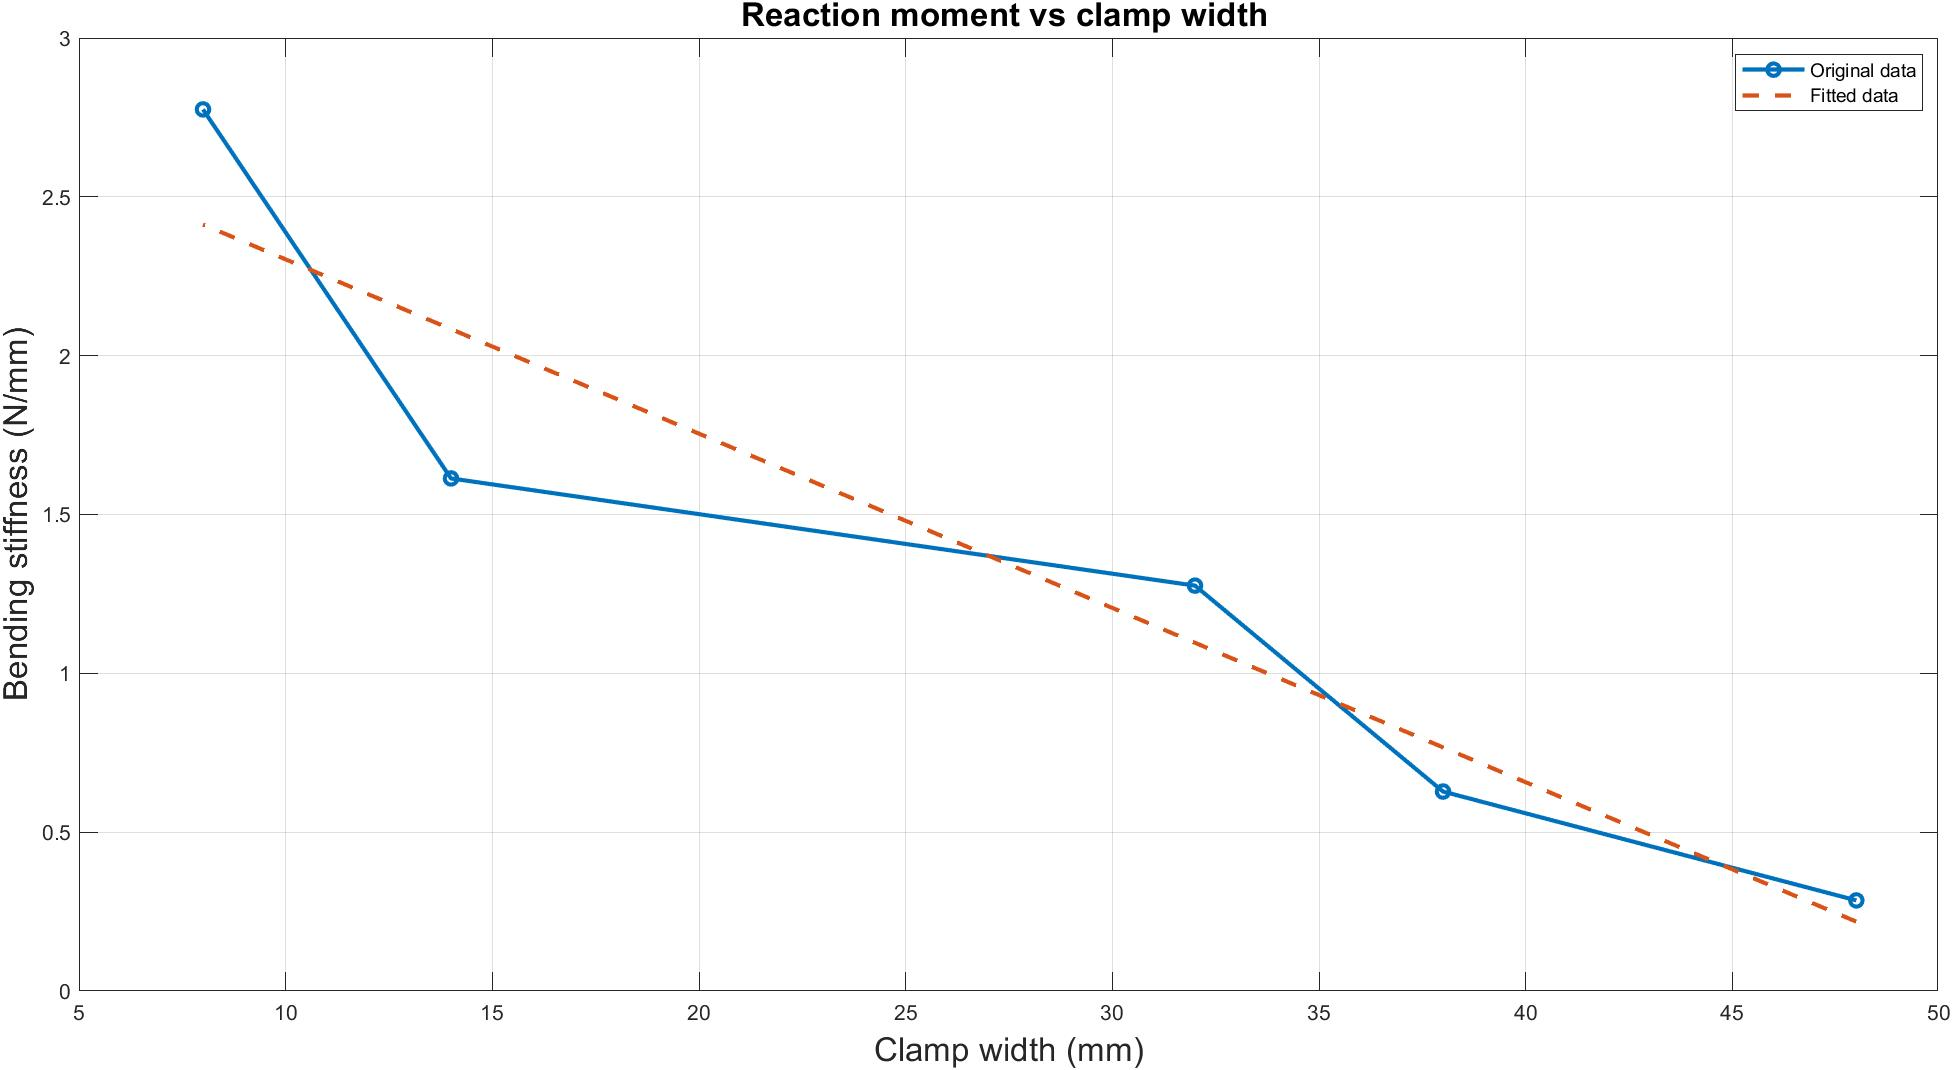
\includegraphics[width=15cm]{images/bend_stiffness.jpg}
    \caption{Bending stiffness plotted against clamp width}
    \label{fig:bendstiff}
\end{figure}
Plot \ref{fig:bendstiff} establishes the bending stiffness against clamp width and it can be seen that the bending stiffness varies almost linearly with the bending stiffness. The equation showing the following linear fit is given by equation \ref{eq:bendstiff} which is the same as equation \ref{eq:maxRM}. 
\begin{equation}
     K=-2.87\times W+ 164.24
     \label{eq:bendstiff}
 \end{equation}
 
    %\input{discussion}
    \section{Conclusion}
\label{sec:conclusion}
This project aims to find the effects of changing the clamp widths on the load bearing capabilities of a deployable boom to accurately estimate the limits of the boom and thereby predict the buckling of the boom. This is necessary as the booms are attached to a cylindrical canister using two screws, and not the typical encastered condition in which the whole of root is assumed to be fixed. These conditions are modelled using various downwards displacement to obtain a fixed width on the boom. Changing the clamp widths has effects on the ploy length which is defined to be 5\% magnitude of the undeformed width of the boom and also the rotational moment on the tip. The clamp width is related to the ploy length with a second order relationship and the maximum rotational moment is related to the clamp width with a linear relationship. 
From the simulation it was found that the boom bends slightly inwards but to an almost constant extent for all the cases. The reasons for this are not yet clear but can be looked in the future. It would be interesting to note the effects of rotational moment in the opposite sense bending with varying clamp widths and compare the relationship with change in clamp width. An ABAQUS script could also be made in order to give more data points which can confirm these relationships. The increasing propagation moments with a decrease in clamp widths can also be explored. Another solution developed in reference \cite{Footdale2014} is a deployment mechanism with a clearance cut of the boom. This allows for a narrower width of a boom, however it would be useful to study the trade-offs of this method given that a narrower boom might result in a lower bending stiffness. 


    
    \small{
	\bibliographystyle{ieeetr}
	\bibliography{fyp.bib}
	}
	\newpage
\appendix
\section{FEA model: Vertical displacements of boundary conditions}
\begin{table}[!hbt]
\centering
\begin{tabular}{|l|l|}
\hline
\textbf{Width of mesh} & \textbf{Displacement(mm)} \\ \hline
1 & 0.03 \\ \hline
2 & 0.13 \\ \hline
3 & 0.29 \\ \hline
4 & 0.51 \\ \hline
5 & 0.80 \\ \hline
6 & 1.14 \\ \hline
7 & 1.55 \\ \hline
8 & 2.01 \\ \hline
9 & 2.53 \\ \hline
10 & 3.10 \\ \hline
11 & 3.72 \\ \hline
12 & 4.39 \\ \hline
13 & 5.11 \\ \hline
14 & 5.87 \\ \hline
15 & 6.67 \\ \hline
16 & 7.50 \\ \hline
17 & 8.37 \\ \hline
18 & 9.26 \\ \hline
19 & 10.18 \\ \hline
20 & 11.12 \\ \hline
21 & 12.07 \\ \hline
22 & 13.04 \\ \hline
23 & 14.02 \\ \hline
24 & 15.00 \\ \hline
\end{tabular}
\caption{Displacements used to flatten the root}
\label{tab:disp}
\end{table}

\begin{figure}[!hbt]
     \centering
     \begin{subfigure}[b]{0.4\textwidth}
         \centering
         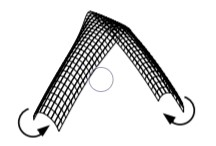
\includegraphics[width=\textwidth]{images/samesense.JPG}
         \caption{Same-sense bending of tapespring}
         \label{fig:same}
     \end{subfigure}
     \hfill
     \begin{subfigure}[b]{0.4\textwidth}
         \centering
         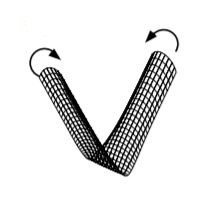
\includegraphics[width=\textwidth]{images/oppsense.JPG}
         \caption{Opposite-sense bending of tapespring}
         \label{fig:opp}
     \end{subfigure}
     \caption{Bending conventions}
     \end{figure}

\newpage
\section{Fitted curves error for ploy lengths}
\begin{table}[!hbt]
\centering
\begin{tabular}{|ll|l|l|l|l|}
\cline{3-6}
\multicolumn{1}{c}{} & \multicolumn{1}{c|}{} & \multicolumn{2}{c|}{\textbf{First order}} & \multicolumn{2}{c|}{\textbf{Second order}} \\ \hline
\multicolumn{1}{|c|}{\textbf{\begin{tabular}[c]{@{}c@{}}Clamp width \\ (mm)\end{tabular}}} &
\multicolumn{1}{c|}{\textbf{\begin{tabular}[c]{@{}c@{}}Ploy length \\ (mm)\end{tabular}}} & \multicolumn{1}{c|}{\textbf{\begin{tabular}[c]{@{}c@{}}Curve fit \\ values\end{tabular}}} & \multicolumn{1}{c|}{\textbf{\begin{tabular}[c]{@{}c@{}}Fit error \\ percentage\end{tabular}}} & \multicolumn{1}{c|}{\textbf{\begin{tabular}[c]{@{}c@{}}Curve fit\\  values\end{tabular}}} & \multicolumn{1}{c|}{\textbf{\begin{tabular}[c]{@{}c@{}}Fit error \\ percentage\end{tabular}}} \\ \hline
\multicolumn{1}{|l|}{45.16} & 197.00 & 216.49 & 9.89 & 191.67 & -2.71 \\ \hline
\multicolumn{1}{|l|}{43.20} & 197.00 & 211.60 & 7.41 & 193.26 & -1.90 \\ \hline
\multicolumn{1}{|l|}{41.23} & 196.00 & 206.71 & 5.47 & 194.26 & -0.89 \\ \hline
\multicolumn{1}{|l|}{39.27} & 195.00 & 201.83 & 3.50 & 194.67 & -0.17 \\ \hline
\multicolumn{1}{|l|}{37.31} & 193.00 & 196.94 & 2.04 & 194.49 & 0.77 \\ \hline
\multicolumn{1}{|l|}{35.34} & 191.00 & 192.05 & 0.55 & 193.72 & 1.42 \\ \hline
\multicolumn{1}{|l|}{33.38} & 190.00 & 187.17 & -1.49 & 192.37 & 1.25 \\ \hline
\multicolumn{1}{|l|}{31.42} & 187.00 & 182.28 & -2.52 & 190.42 & 1.83 \\ \hline
\multicolumn{1}{|l|}{29.45} & 184.00 & 177.39 & -3.59 & 187.89 & 2.11 \\ \hline
\multicolumn{1}{|l|}{27.49} & 179.00 & 172.51 & -3.63 & 184.77 & 3.22 \\ \hline
\multicolumn{1}{|l|}{25.53} & 180.00 & 167.62 & -6.88 & 181.06 & 0.59 \\ \hline
\multicolumn{1}{|l|}{23.56} & 171.00 & 162.73 & -4.83 & 176.76 & 3.37 \\ \hline
\multicolumn{1}{|l|}{21.60} & 172.00 & 157.85 & -8.23 & 171.88 & -0.07 \\ \hline
\multicolumn{1}{|l|}{19.63} & 163.00 & 152.96 & -6.16 & 166.40 & 2.09 \\ \hline
\multicolumn{1}{|l|}{17.67} & 162.00 & 148.08 & -8.60 & 160.34 & -1.03 \\ \hline
\multicolumn{1}{|l|}{15.71} & 154.00 & 143.19 & -7.02 & 153.69 & -0.20 \\ \hline
\multicolumn{1}{|l|}{13.74} & 149.00 & 138.30 & -7.18 & 146.44 & -1.72 \\ \hline
\multicolumn{1}{|l|}{11.78} & 145.00 & 133.42 & -7.99 & 138.61 & -4.40 \\ \hline
\multicolumn{1}{|l|}{9.82} & 128.00 & 128.53 & 0.41 & 130.20 & 1.72 \\ \hline
\multicolumn{1}{|l|}{7.85} & 128.00 & 123.64 & -3.40 & 121.19 & -5.32 \\ \hline
\multicolumn{1}{|l|}{5.89} & 131.00 & 118.76 & -9.35 & 111.60 & -14.81 \\ \hline
\multicolumn{1}{|l|}{3.93} & 109.00 & 113.87 & 4.47 & 101.41 & -6.96 \\ \hline
\multicolumn{1}{|l|}{1.96} & 106.00 & 108.98 & 2.81 & 90.64 & -14.49 \\ \hline
\end{tabular}
\caption{Error percentage of first order and second order curves}
\end{table}
\section{Maximum reaction moment for changing width of clamp}
\begin{table}[!hbt]
\centering
\begin{tabular}{|c|c|}
\hline
\multicolumn{1}{|c|}{\textbf{\begin{tabular}[c]{@{}c@{}}Width of \\ the clamp (mm)\end{tabular}}} & \multicolumn{1}{c|}{\textbf{\begin{tabular}[c]{@{}c@{}}Maximum reaction \\ moment\ (Nmm)\end{tabular}}} \\ \hline
48 & 31.5 \\ \hline
38 & 47.7 \\ \hline
32 & 78.5 \\ \hline
14 & 105 \\ \hline
8 & 157 \\ \hline
\end{tabular}
\caption{\label{tab:rotwidth}Maximum reaction moment and width of the clamp}
\end{table}

\newpage
\section{Calladine shell theory}
\begin{figure}[!hbt]
    \centering
    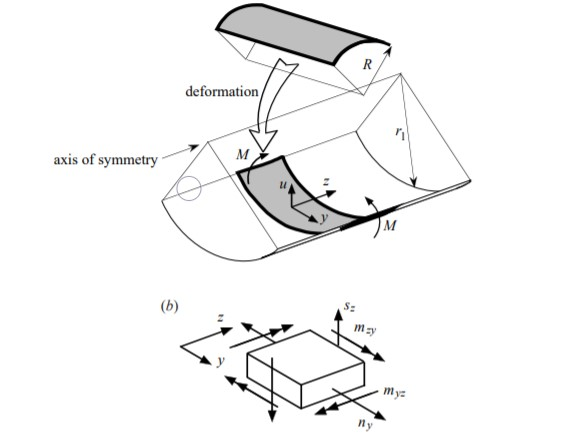
\includegraphics{images/mansfieldtheory.jpg}
    \caption{Calladine shell theory from source \cite{Seffen1999}}
    \label{fig:mansfield}
\end{figure}

\begin{figure}[!hbt]
    \centering
    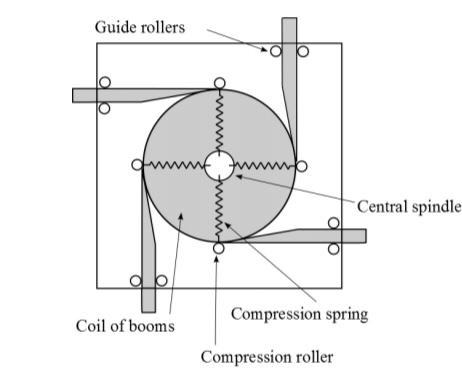
\includegraphics[height=6cm]{images/guiderollers.jpg}
    \caption{Position of guiderollers in STEM boom deployers from source \cite{Hoskin2015}}
    \label{fig:guiderollers}
\end{figure}



	
\end{document}


